\chapter{Experimenty za~účelem zlepšení identifikace}
\label{chp:exps}

Tato kapitola představuje soubor experimentů zaměřených na~zefektivnění procesu identifikace aplikací. Hlavním cílem je minimalizace mohutnosti kandidátní množiny aplikací při~současném zachování co nejvyšší přesnosti. Zároveň jsou respektovány všechny relevantní nefunkční požadavky, zejména s~ohledem na~časovou náročnost.

Identifikace a~použití otisků probíhá ve dvou fázích, jak bylo popsáno v~sekci~\ref{sub:architecture}. Nejprve je aplikována metoda fingerprintingu \textit{JA3}, \textit{JA4} či jejich kombinace, na~jejímž základě je získána kandidátní množina (proběhne jednoduché vyhledání aplikací, které odpovídají danému otisku). Tato množina kandidátů je dále v~textu označována jako \textbf{počáteční kandidátní množina}.

Počáteční kandidátní množina přímo určuje, které získané vzory (tj. vzory získané z~trénovací množiny) se budou používat pro~výpočet podobnosti. V~modelové situaci je pro~dané spojení vygenerována počáteční kandidátní množina obsahující \texttt{App1}, \texttt{App2} a~\texttt{App3}. Výpočet podobnosti mezi~kontextem daného spojení a~frekventovanými vzory tedy probíhá pouze pro~vzory aplikací \texttt{App1}, \texttt{App2} a~\texttt{App3}.

Tímto způsobem se zefektivní identifikace aplikací, jelikož není potřeba iterovat přes časté vzory, které nejsou v~počáteční kandidátní množině. Použití kontextu zde slouží pouze ke~zúžení kandidátní množiny. Tato množina bude dále v~textu označována jako \textbf{finální kandidátní množina}.

\section{Volby položek pro~získání vzorů}
\label{sec:ex1}
Cílem tohoto experimentu je vyhodnotit, které otisky a~případně další atributy spojení, například \textit{SNI} či \textit{ORG}, přinášejí nejvyšší přesnost identifikace, a~to jak při~tvorbě počáteční kandidátní množiny, tak i~jako vstupní data pro~algoritmus \textit{Apriori}. Ideální kombinace by zároveň měla generovat co nejkratší finální kandidátní množinu aplikací a~udržet výpočetní náročnost v~přijatelných mezích.

Pro tyto experimenty byly ostatní parametry zvoleny následovně: \textbf{minimální podpora} algoritmu \textit{Apriori} byla nastavena \textbf{na 0{,}25}, \textbf{počet finálních kandidátů na~3}, \textbf{šířka okna na~15} spojení u~sady \texttt{iscx.csv} a~\textbf{25} u~sady \texttt{mobile-desktop-apps-raw.csv}. Metody generující počáteční kandidátní množinu byly: \textit{JA3}, \textit{JA3+JA3S+SNI}, \textit{JA4} a~\textit{JA4+JA4S+SNI}.

Tabulka \ref{tab:fingerprints-accuracy} shrnuje přesnost a~průměrnou délku počáteční kandidátní množiny po~aplikaci metod \textit{JA3}, \textit{JA4} a~jejich kombinací. Výsledky odpovídají čistému fingerprintingu daných spojení, tedy bez~využití kontextu a~frekventovaných vzorů. Tabulka slouží jako výchozí přehled přesnosti základního fingerprintingu na~jednotlivých datových sadách a~jako referenční bod pro~následné porovnání s~výsledky identifikace využívající kontext. 

\begin{table}[H]
	\centering
	\begin{tabular}{lrrrr}
		\toprule
		\multirow{2}*{\textbf{Otisky}}&\multicolumn{2}{c}{\texttt{iscx.csv}} & \multicolumn{2}{c}{\texttt{mobile\_desktop\_apps\_raw.csv}} \\
		             & \textbf{Přesnost} & \textbf{Délka} & \textbf{Přesnost} & \textbf{Délka} \\
		\midrule
		JA3          & 0.975              & 3.146           & 0.495              & 4.325           \\
		JA3+JA3S+SNI & 0.924              & 2.099           & 0.855              & 5.953           \\
		JA4          & 0.975              & 3.146           & 0.966              & 14.298          \\
		JA4+JA4S+SNI & 0.924              & 2.094           & 0.854              & 3.382           \\
		\bottomrule
	\end{tabular}
	\caption{Přesnost otisků a~jejich kombinací}
	\label{tab:fingerprints-accuracy}
\end{table} 

V~následujících tabulkách jsou uvedeny výsledky identifikace s~využitím kontextu a~vzorů. V~záhlaví každé tabulky je vždy uvedena metoda, pomocí které byla určena počáteční kandidátní množina. Kombinace pak specifikuje položky, ze kterých algoritmus \textit{Apriori} získává časté vzory.
Výsledky zahrnují přesnost identifikace, počítanou jako podíl případů, kdy byla správně určena aplikace nacházející se ve~finální kandidátní množině, vůči celkovému počtu identifikovaných spojení. Dále je uvedena délka, která reprezentuje průměrnou velikost finální kandidátní množiny. Je zaznamenán i~čas, potřebný pro~identifikaci, pouze pro~datovou sadu \texttt{mobile-desktop-apps-raw.csv}. Časové hodnoty byly měřeny na~testovacím zařízení s~následujícími parametry: CPU: \texttt{AMD Ryzen 7 5700U (16) @~1.80 GHz}, OS:\texttt{ EndeavourOS x86\_64}, RAM: \texttt{16 GB}. Přestože je časová náročnost závislá na~výkonu konkrétního zařízení, poskytují tyto hodnoty orientační představu o~relativní složitosti jednotlivých variant identifikace. Z~typografických důvodů byla pro~kombinaci položek \textit{JA3+JA3S+JA4+JA4S} zvolena zkratka \textit{JA34S*}. Všechny výsledky testované kombinace položek jsou uvedeny v~příloze~\ref{chp:appendix-experiments}.

\begin{table}[H]
	\centering
	\begin{tabular}{lrr|rrr}
		\toprule
		\multicolumn{6}{c}{\textbf{Počáteční kandidátní množina získaná pomocí metody \textit{JA3} }} \\
		\midrule
		\multirow{2}*{\textbf{Kombinace položek}}&\multicolumn{2}{c}{\texttt{iscx.csv}} & \multicolumn{3}{c}{\texttt{mobile\_desktop\_apps\_raw.csv}} \\
		               & \textbf{Přesnost} & \textbf{Délka} & \textbf{Přesnost} & \textbf{Délka} & \textbf{Čas [s]} \\
		\midrule
		JA3            & 0.837              & 2.128           & 0.279              & 2.778           & 74.470           \\
		JA4            & 0.837              & 2.128           & 0.390              & 2.792           & 60.340           \\
		JA4+JA4S       & 0.842              & 2.128           & 0.487              & 2.796           & 112.910          \\
		JA3+JA3S+SNI   & 0.852              & 2.128           & 0.371              & 2.796           & 163.680          \\
		JA4+JA4S+SNI   & 0.847              & 2.128           & 0.490              & 2.796           & 185.050          \\
		JA34S*+SNI     & 0.842              & 2.128           & 0.441              & 2.796           & 575.500          \\
		JA34S*+SNI+ORG & 0.849              & 2.128           & 0.423              & 2.796           & 1123.730         \\
																		
		\bottomrule
	\end{tabular}
	\caption{Výsledky experimentu s~kombinacemi položek, které byly použity jako vstupní data pro~získání častých vzorů pomocí algoritmu \textit{Apriori}, při~použití počáteční kandidátní množiny získané pomocí metody \textit{JA3}.}
	\label{tab:merged-not_comb-accuracy-ja3}
\end{table}

V první části experimentu, při~použití metody \textit{JA3} pro~generování počáteční kandidátní množiny jsou výsledky uvedeny v~tabulce~\ref{tab:merged-not_comb-accuracy-ja3}. U~datové sady \texttt{iscx.csv} dosahuje většina kombinací přesnosti kolem 0{,}84, přičemž průměrná délka finální kandidátní množiny činí 2{,}128 kandidátů na~spojení, a~to i~bez~výrazného navýšení počtu položek. 

Naproti tomu \texttt{mobile\_desktop\_apps\_raw.csv} vykazuje výrazně nižší přesnost identifikace. Ačkoliv kombinace \textit{JA4+JA4S+SNI} dosahuje obdobné přesnosti jako samotné použití otisku \textit{JA3} (0{,}490 při~délce 2{,}796 oproti 0{,}495 při~délce 4{,}325), jak je uvedeno v~tabulce~\ref{tab:fingerprints-accuracy}, ukazuje se, že tato datová sada je \textbf{mnohem citlivější na~volbu kombinace otisků}. Rozdíl mezi~nejhorším a~nejlepším výsledkem činí \textbf{0{,}211}, což poukazuje na~značný dopad správného výběru položek na~výslednou přesnost.

Při použití metody \textit{JA4} pro~vytváření počáteční kandidátní množiny jsou výsledky uvedené v~tabulce~\ref{tab:merged-not_comb-accuracy-ja4}, pro~datovou sadu \texttt{iscx.csv}, identické s~výsledky dosaženými při~použití počáteční množiny vytvořené pomocí \textit{JA3} (viz.Tabulka~\ref{tab:merged-not_comb-accuracy-ja3}). V~případě této datové sady tedy zvolená metoda pro~získaní počáteční kandidátní množiny nemá vliv na~výslednou úspěšnost identifikace. Tento jev lze pravděpodobně přičíst nižšímu počtu různých aplikací.

\begin{table}[H]
	\centering
	\begin{tabular}{lrr|rrr}
		\toprule
		\multicolumn{6}{c}{\textbf{Počáteční kandidátní množina získaná pomocí metody \textit{JA4}}} \\
		\midrule
		\multirow{2}*{\textbf{Kombinace položek}}&\multicolumn{2}{c}{\texttt{iscx.csv}} & \multicolumn{3}{c}{\texttt{mobile\_desktop\_apps\_raw.csv}} \\
		               & \textbf{Přesnost} & \textbf{Délka} & \textbf{Přesnost} & \textbf{Délka} & \textbf{Čas [s]} \\
		\midrule
		JA3            & 0.837              & 2.128           & 0.304              & 2.781           & 53.660           \\
		JA4            & 0.837              & 2.128           & 0.387              & 2.785           & 32.340           \\
		JA4+JA4S       & 0.842              & 2.128           & 0.558              & 2.791           & 58.500           \\
		JA3+JA3S+SNI   & 0.852              & 2.128           & 0.489              & 2.791           & 66.340           \\
		JA4+JA4S+SNI   & 0.847              & 2.128           & 0.548              & 2.791           & 84.030           \\
		JA34S*+SNI     & 0.842              & 2.128           & 0.549              & 2.791           & 225.220          \\
		JA34S*+SNI+ORG & 0.849              & 2.128           & 0.533              & 2.791           & 400.770          \\
																		
		\bottomrule
	\end{tabular}
	\caption{Výsledky experimentu s~kombinacemi položek, které byly použity jako vstupní data pro~získání častých vzorů pomocí algoritmu \textit{Apriori}, při~použití počáteční kandidátní množiny získané pomocí metody \textit{JA4}.}
	\label{tab:merged-not_comb-accuracy-ja4}
\end{table}

U druhé datové sady došlo oproti předchozí metodě k~mírnému zlepšení přesnosti identifikace. Přesto však i~s~nejpřesnější kombinací \textit{JA3+JA3S+JA4+JA4S} je dosaženo pouze přesnosti 0{,}577 při~průměrné délce finální kandidátní množiny 2{,}791, zatímco při~použití samotného fingerprintingu pomocí \textit{JA4} je dosaženo výrazně vyšší přesnosti 0{,}975, i~když za~cenu výrazně delší průměrné kandidátní množiny 14{,}298 (viz. Tabulka~\ref{tab:fingerprints-accuracy}). 

Přesnost identifikace při~využití metody \textit{JA3+JA3S+SNI} pro~získání počáteční kandidátní množiny vykazuje výrazné zlepšení, zejména u~druhé datové sady (viz. Tabulka~\ref{tab:merged-comb-accuracy-ja3}). 

Nejvíce se to projevuje u~kombinací \textit{JA4+JA4S} a~\textit{JA4+JA4S+SNI}, kde přesnost identifikace dosahuje hodnoty \textbf{0{,}800} při~průměrné délce finální kandidátní množiny \textbf{1{,}734}. Tato přesnost se tak výrazně přibližuje hodnotě 0{,}855 dosažené při~použití fingerprintingu, avšak při~podstatně větší průměrné délce kandidátní množiny 5{,}953, jak je uvedeno v~Tabulce~\ref{tab:fingerprints-accuracy}. Toto zlepšení však přináší vyšší dobou trvání identifikace. 

Tento přístup zároveň přináší mírné zlepšení také u~datové sady \texttt{iscx.csv}, kde průměrná délka kandidátní množiny \textbf{klesá z~2{,}128 na~1{,}583} kandidátů.

\begin{table}[H]
	\centering
	\begin{tabular}{lrr|rrr}
		\toprule
		\multicolumn{6}{c}{\textbf{Počáteční kandidátní množina získaná pomocí metody\textit{ JA3+JA3S+SNI}}} \\
		\midrule
		\multirow{2}*{\textbf{Kombinace položek}}&\multicolumn{2}{c}{\texttt{iscx.csv}} & \multicolumn{3}{c}{\texttt{mobile\_desktop\_apps\_raw.csv}} \\
		               & \textbf{Přesnost} & \textbf{Délka} & \textbf{Přesnost} & \textbf{Délka} & \textbf{Čas [s]} \\
		\midrule
		JA3            & 0.867              & 1.583           & 0.385              & 2.287           & 74.470           \\
		JA4            & 0.867              & 1.583           & 0.771              & 1.747           & 60.340           \\
		JA4+JA4S       & 0.869              & 1.583           & 0.800              & 1.734           & 112.910          \\
		JA3+JA3S+SNI   & 0.872              & 1.583           & 0.790              & 1.734           & 163.680          \\
		JA4+JA4S+SNI   & 0.867              & 1.583           & 0.798              & 1.734           & 185.050          \\
		JA34S*+SNI     & 0.867              & 1.583           & 0.792              & 1.734           & 575.500          \\
		JA34S*+SNI+ORG & 0.869              & 1.583           & 0.774              & 1.734           & 1123.730         \\
																		
		\bottomrule
	\end{tabular}
	\caption{Výsledky experimentu s~kombinacemi položek, které byly použity jako vstupní data pro~získání častých vzorů pomocí algoritmu \textit{Apriori}, při~použití počáteční kandidátní množiny získané pomocí metody\textit{JA3+JA3S+SNI}.}
	\label{tab:merged-comb-accuracy-ja3}
\end{table}

Tabulka~\ref{tab:merged-comb-accuracy-ja4} uvádí výsledky identifikace s~počáteční kandidátní množinou generovanou použitím kombinace \textit{JA4+JA4S+SNI}. Přesnost a~průměrná délka finální kandidátní množiny vykazují \textbf{mírné zlepšení} oproti dříve uvedeným metodám, hlavním přínosem této kombinace je však \textbf{výrazně kratší doba trvání} identifikace -- ve~srovnání s~kombinací \textit{JA3+JA3S+SNI} je přibližně poloviční, v~některých případech dokonce až třetinová. 

\begin{table}[H]
	\centering
	\begin{tabular}{lrr|rrr}
		\toprule
		\multicolumn{6}{c}{\textbf{Počáteční kandidátní množina získaná pomocí metody \textit{JA4+JA4S+SNI}}} \\
		\midrule
		\multirow{2}*{\textbf{Kombinace položek}}&\multicolumn{2}{c}{\texttt{iscx.csv}} & \multicolumn{3}{c}{\texttt{mobile\_desktop\_apps\_raw.csv}} \\
		               & \textbf{Přesnost} & \textbf{Délka} & \textbf{Přesnost} & \textbf{Délka} & \textbf{Čas [s]} \\
		\midrule
		JA3            & 0.869              & 1.585           & 0.385              & 2.277           & 53.660           \\
		JA4            & 0.869              & 1.585           & 0.770              & 1.727           & 32.340           \\
		JA4+JA4S       & 0.869              & 1.585           & 0.798              & 1.714           & 58.500           \\
		JA3+JA3S+SNI   & 0.874              & 1.585           & 0.795              & 1.714           & 66.340           \\
		JA4+JA4S+SNI   & 0.869              & 1.585           & 0.804              & 1.714           & 84.030           \\
		JA34S*+SNI     & 0.869              & 1.585           & 0.797              & 1.714           & 225.220          \\
		JA34S*+SNI+ORG & 0.872              & 1.585           & 0.782              & 1.714           & 400.770          \\
																		
		\bottomrule
	\end{tabular}
	\caption{Výsledky experimentu s~kombinacemi položek, které byly použity jako vstupní data pro~získání častých vzorů pomocí algoritmu \textit{Apriori}, při~použití počáteční kandidátní množiny získané pomocí metody \textit{JA4+JA4S+SNI}.}
	\label{tab:merged-comb-accuracy-ja4}
\end{table}

Hlavním důvodem tohoto zrychlení je nižší počet kandidátních aplikací (mohutnost počáteční kandidátní množiny je menší viz. Tabulka~\ref{tab:fingerprints-accuracy}), a~tedy i~menší množství vzorů, které je potřeba porovnat. Při~použití fingerprintingu s~kombinací \textit{JA4+JA4S+SNI} bez~kontextu nad~datovou sadou \texttt{mobile\_desktop\_apps\_raw.csv} je dosaženo přesnosti 85{,}4\% při~průměrné délce kandidátní množiny 3{,}382. Při~identifikaci využívající kontext \textbf{klesá přesnost přibližně o~5\%}, avšak průměrná délka finální kandidátní množiny je \textbf{více než poloviční}.

Testování identifikace s~různými položkami a~jejich kombinacemi přineslo cenný pohled na~jejich využitelnost. Experiment byl rovněž proveden s~položkou \textit{ClientExtension}, avšak vzhledem k~tomu, že tato položka nepřinesla žádné významné zlepšení, není zde podrobně uvedena. Podrobné výsledky lze nalézt v~příloze~\ref{sec:appendix:ex1}.

Na základě provedených experimentů se jako nejefektivnější pro~identifikaci aplikací pomocí kontextu ukazují otisky \textit{JA4} a~jejich kombinace. Tyto kombinace se osvědčily jak při~vyhledávání v~kontextu, tak při~generování počáteční kandidátní množiny. Mezi~nejlépe hodnocené kombinace pro~získávání častých vzorů patří: \textit{JA4+JA4S}, \textit{JA4+JA4S+SNI} a~\textit{JA3+JA4} v~kombinaci s~metodami \textit{JA4} a~\textit{JA4+JA4S+SNI} pro~generování počáteční kandidátní množiny. Tyto přístupy dosahují nejvyšší přesnosti identifikace při~zachování kratší délky kandidátní množiny a~zároveň přispívají k~výraznému zkrácení doby trvání identifikace.

\section{Minimální podpora algoritmu \textit{Apriori}}
\label{ex-min_sup}
Tento experiment zkoumá závislost mezi~volbou minimální podpory algoritmu \textit{Apriori}, přesností identifikace a~průměrnou délkou finální kandidátní množiny. Testování probíhá nad~třemi nejlépe hodnocenými kombinacemi otisků z~předchozího experimentu popsaného v~sekci~\ref{sec:ex1}, konkrétně \textit{JA3+JA4}, \textit{JA4+JA4S+SNI} a~\textit{JA4+JA4S} v~kombinaci s~metodou \textit{JA4+JA4S+SNI} pro~generování počáteční kandidátní množiny.

Cílem je určit, jak výrazně výběr prahové hodnoty podpory ovlivňuje kvalitu výsledné množiny kandidátů. Příliš vysoká hodnota podpory může vést k~zanedbání užitečných, avšak méně frekventovaných vzorů, zatímco příliš nízká může zahrnout i~irelevantní kombinace, čímž může narůstat velikost kandidátní množiny a~zvyšuje se výpočetní náročnost. Výsledky experimentu by tak měly napomoci při~optimalizaci nastavení algoritmu.

\begin{figure}[H]
	\centering
	\begin{minipage}[t]{0.49\textwidth}
		\centering
		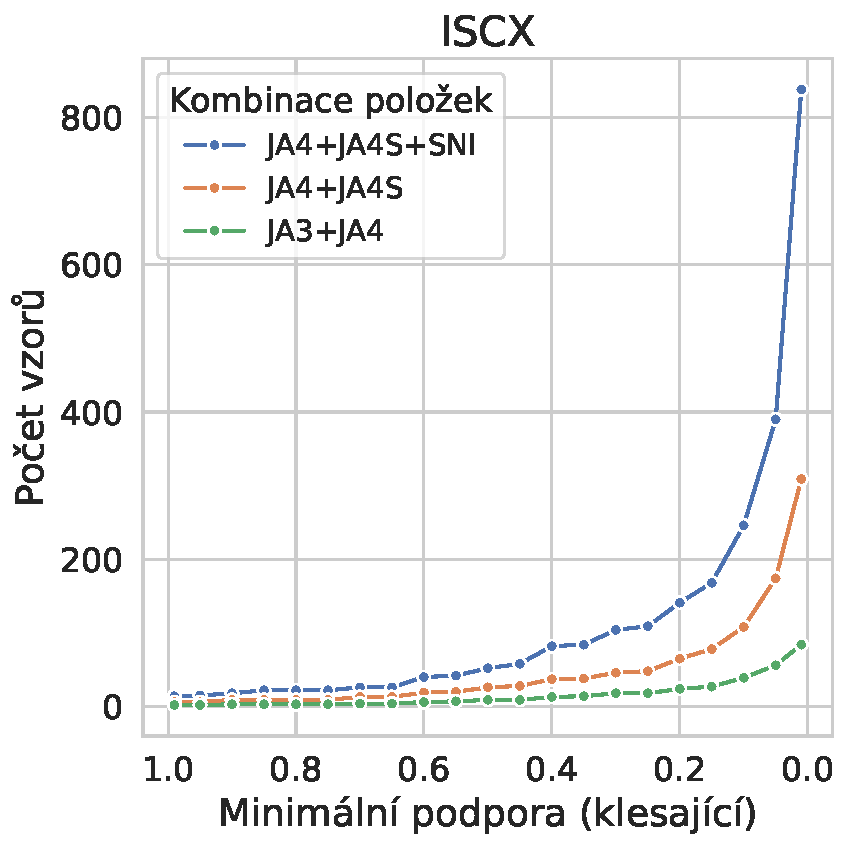
\includegraphics[width=\linewidth]{obrazky-figures/exps/ex2-num_patterns-iscx.pdf}
		\caption{Počet vzorů v~závislosti na~podpoře pro~\texttt{iscx.csv}.}
		\label{fig:ex2-iscx-patterns}
	\end{minipage}%
	\hfill
	\begin{minipage}[t]{0.49\textwidth}
		\centering
		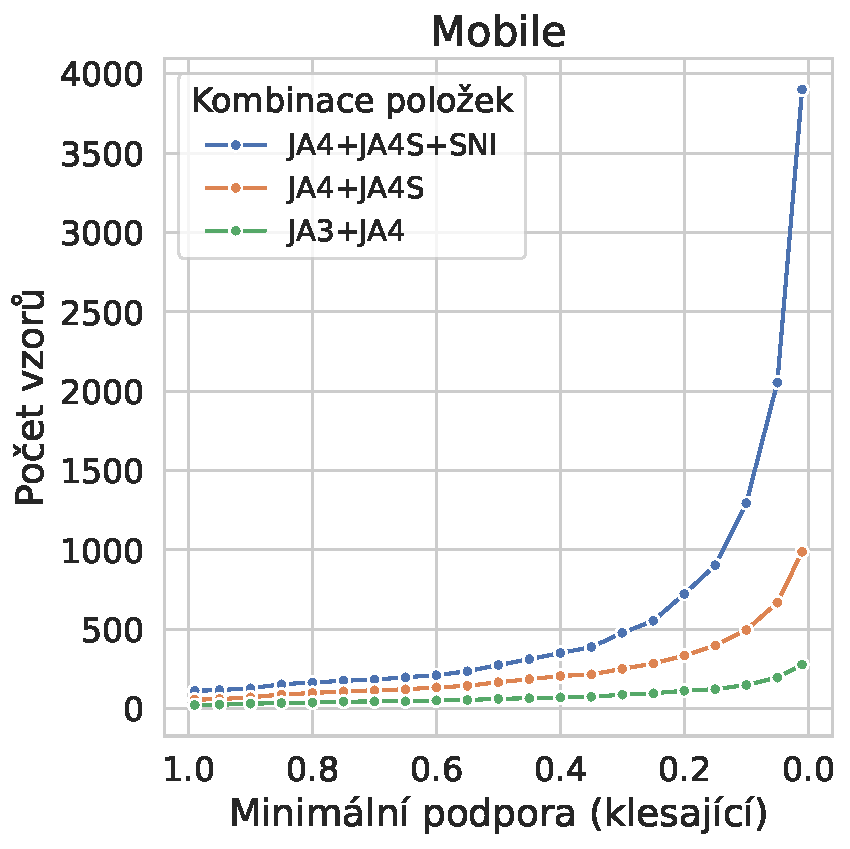
\includegraphics[width=\linewidth]{obrazky-figures/exps/ex2-num_patterns-mobile.pdf}
		\caption{Počet vzorů v~závislosti na~podpoře pro~\texttt{mobile\_desktop\_apps\_raw.csv}.}
		\label{fig:ex2-mobile-patterns}
	\end{minipage}
\end{figure}

Ostatní parametry pro~tento experiment byly nastaveny následovně: \textbf{šířka okna 15 spojení}, maximální \textbf{počet finálních kandidátů na~3}.

Je zřejmé, že volba minimální podpory přímo ovlivňuje počet identifikovaných vzorů v~rámci okolních spojení, jak ilustruje graf na~obrázku~\ref{fig:ex2-iscx-patterns} pro~datovou sadu \texttt{iscx.csv} a~graf na~obrázku~\ref{fig:ex2-mobile-patterns} pro~datovou sadu \texttt{mobile\_desktop\_apps\_raw.csv}. Lze rovněž očekávat, že celkový počet vzorů výrazně narůstá s~velikostí datové sady, což potvrzuje sada \texttt{mobile\_desktop\_apps\_raw.csv}, kde zaznamenaný počet vzorů \textbf{při minimální podpoře 0{,}01 dosahuje téměř 4000}. Naproti tomu u~sady \texttt{iscx.csv} celkový počet vzorů mírně \textbf{přesahuje hodnotu 800}.

V obou datových sadách je přesnost identifikace při~nastavení minimální podpory v~intervalu $(0{,}30; 0{,}99\rangle$ poměrně nízká a~roste s~klesající hodnotou podpory. V~nejlepších případech dosahuje maximálně hodnoty 0{,}7. Při~podpoře \textbf{nižší než 0{,}3} vykazují obě datové sady výrazně lepší úroveň identifikace.
\begin{figure}[H]
	\centering
	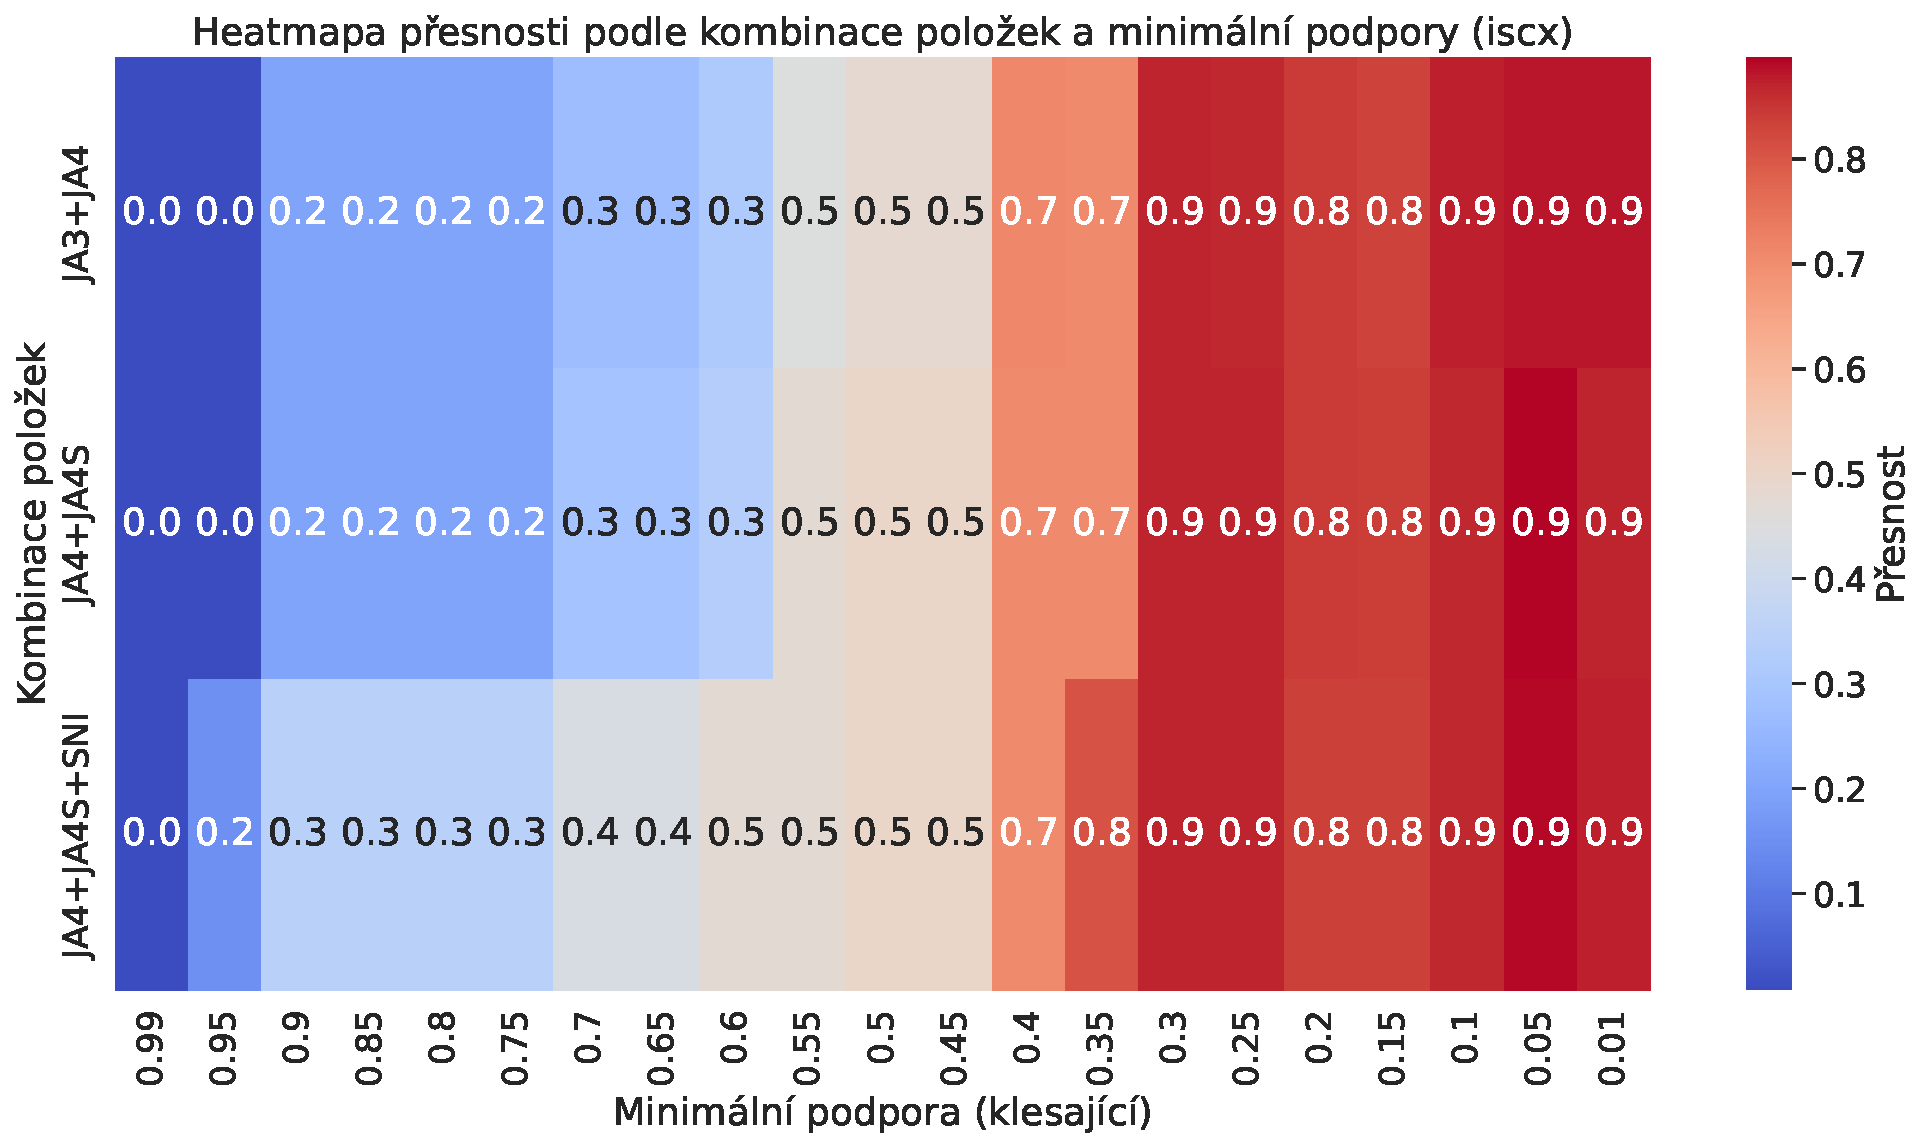
\includegraphics[width=\textwidth]{obrazky-figures/exps/ex2-iscx-heatmap.pdf}
	\caption{Heatmapa znázorňuje testované kombinace položek pro~algoritmus \textit{Apriori} v~závislosti na~volbě minimální podpory a~dosažené přesnosti pro~datovou sadu \texttt{iscx.csv}, při~použití metody \textit{JA4+JA4S+SNI} pro~nalezení počáteční kandidátní množiny.}
	\label{fig:ex2-iscx-heatmap}
\end{figure}
U datové sady \texttt{iscx.csv} (viz.obr.~\ref{fig:ex2-iscx-heatmap}) lze pozorovat, že všechny testované kombinace dosahují nejvyšší míry identifikace při~hodnotách podpory 0{,}3, 0{,}25 a~0{,}05. Druhá datová sada \texttt{mobile\_desktop\_apps\_raw.csv} (viz.obr.~\ref{fig:ex2-mobile-heatmap}) si od~podpory 0{,}3 udržuje podobnou úroveň přesnosti napříč všemi kombinacemi. Nejlepších výsledků však dosahuje kombinace \textit{JA4+JA4S+SNI} při~hodnotách podpory 0{,}25, 0{,}2, 0{,}05 a~0{,}01. Přesnější identifikace od~těchto hodnot je pravděpodobně způsobena tím, že při~hodnotě 0{,}26 již všechny aplikace mají minimálně jeden vzor.

Experiment byl rovněž proveden s~využitím metody \textit{JA4} pro~generování kandidátní množiny určené k~následné úpravě. Přestože se kombinace \textit{JA4+JA4S+SNI} dosud jeví jako nejvhodnější varianta, výsledky ukazují, že samotný otisk \textit{JA4} zatím nedosahuje požadované úrovně přesnosti. Kompletní výsledky experimentu jsou uvedeny v~příloze~\ref{sec:appendix:ex2}.

\begin{figure}[H]
	\centering
	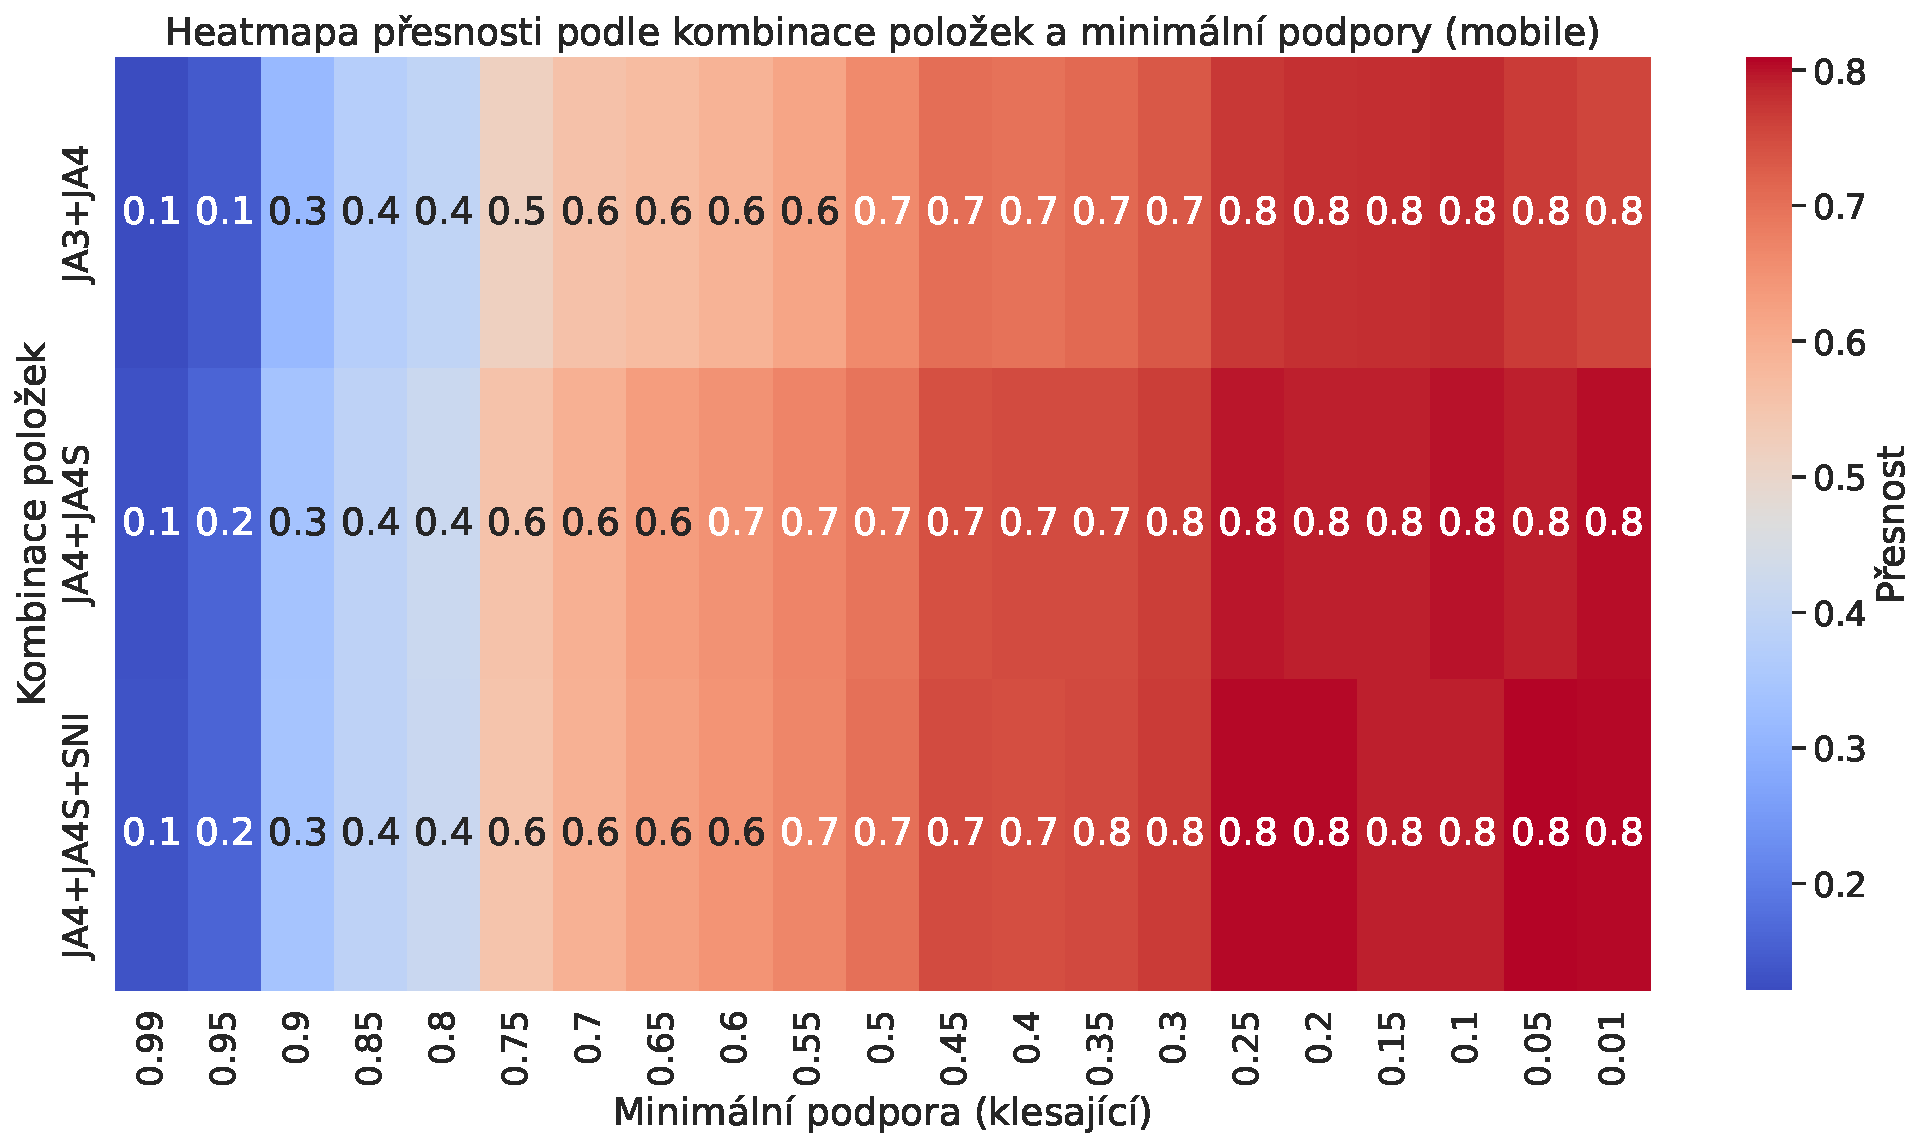
\includegraphics[width=\textwidth]{obrazky-figures/exps/ex2-mobile-heatmap.pdf}
	\caption{Heatmapa zobrazující testované kombinace položek pro~algoritmus \textit{Apriori} v~závislosti na~volbě minimální podpory a~dosažené přesnosti pro~datovou sadu \texttt{mobile desktop apps raw.csv}, při~použití metody \textit{JA4+JA4S+SNI} pro~nalezení počáteční kandidátní množiny.}
	\label{fig:ex2-mobile-heatmap}
\end{figure}

\begin{figure}[H]
	\centering
	\begin{minipage}[t]{0.49\textwidth}
		\centering
		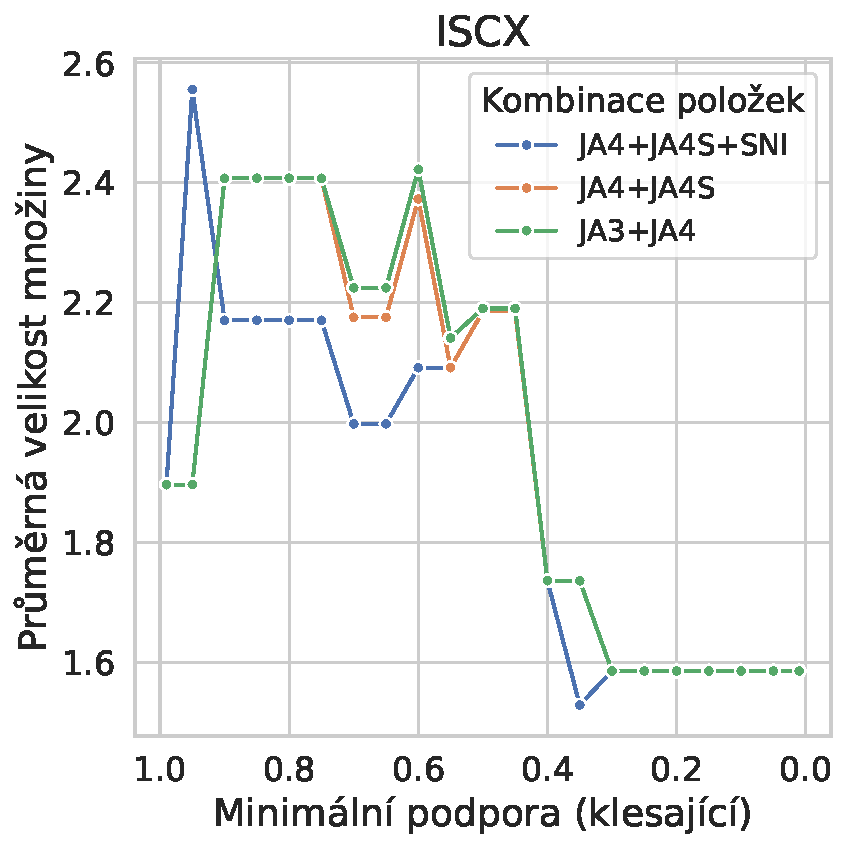
\includegraphics[width=\linewidth]{obrazky-figures/exps/ex2-candidates_len-iscx.pdf}
		\caption{Průměrná velikost finální kandidátní množiny v~závislosti na~podpoře pro~\texttt{iscx csv}.}
		\label{fig:ex2-iscx-candidates}
	\end{minipage}%
	\hfill
	\begin{minipage}[t]{0.49\textwidth}
		\centering
		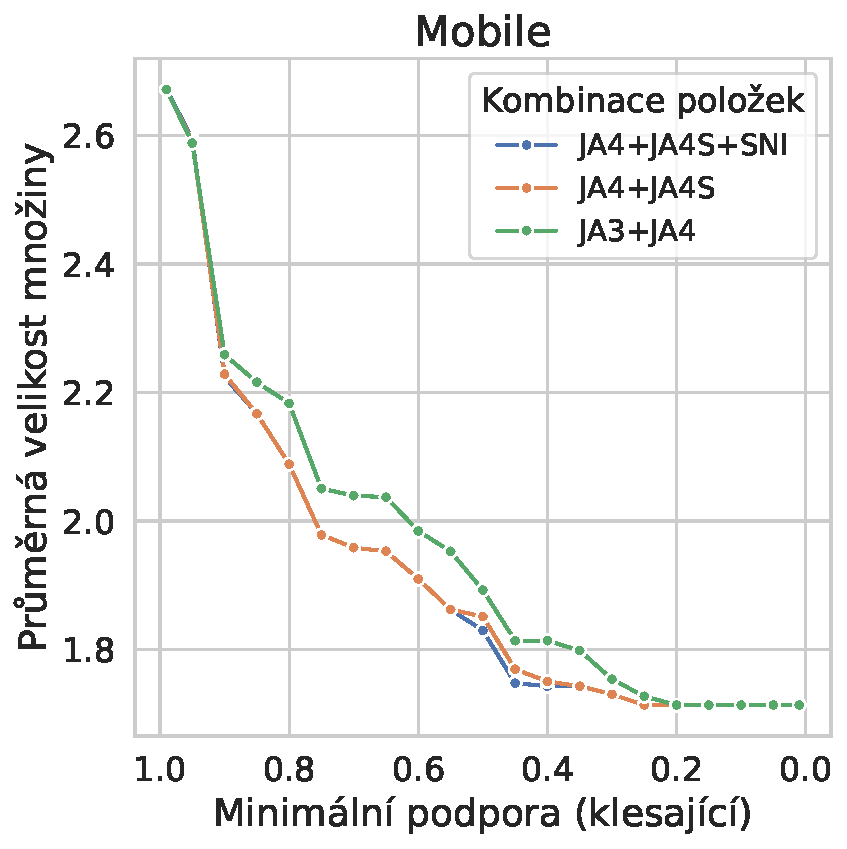
\includegraphics[width=\linewidth]{obrazky-figures/exps/ex2-candidates_len-mobile.pdf}
		\caption{Průměrná velikost finální kandidátní množiny v~závislosti na~podpoře pro~\texttt{mobile desktop apps raw.csv}.}
		\label{fig:ex2-mobile-candidates}
	\end{minipage}
\end{figure}

Průměrná velikost finální kandidátní množiny klesá se snižující se minimální podporou u~obou datových sad. U~datové sady \texttt{iscx.csv} (viz.~graf na~Obrázku~\ref{fig:ex2-iscx-candidates}) jsou rozdíly mezi~jednotlivými kombinacemi výraznější než u~sady \texttt{mobile\_desktop\_apps\_raw.csv} (viz.~graf na~Obrázku~\ref{fig:ex2-mobile-candidates}). Nicméně při~hodnotách podpory 0{,}2 a~nižších konvergují všechny kombinace k~téměř stejné, nejnižší zaznamenané hodnotě (v případě \texttt{iscx.csv} k~druhé nejnižší zaznamenané hodnotě).

V této fázi z~experimentu vyplývá, že nejlepší výsledky v~rámci nastavení minimální podpory se pohybují kolem \textbf{hodnot 0{,}2, 0{,}25 , 0{,}05 nebo 0{,}01}. S~ohledem na~počet vytěžených vzorů se však hodnoty \textbf{0{,}2 a~0{,}25 jeví jako ideální volba} pro~budoucí experimenty. Nabízí totiž srovnatelnou úroveň identifikace jako nižší hodnoty (například 0{,}05), avšak \textbf{s~výrazně menším počtem vzorů}, což snižuje výpočetní náročnost i~složitost následného zpracování.

\subsection{Velikost a~počet vzorů na~aplikaci}
\label{ex-filters}
Tato část představuje druhou fázi experimentu, která se zaměřuje na~analýzu počtu a~délky vzorů přiřazených jednotlivým aplikacím. Cílem je detailněji prozkoumat získané vzory a~jejich vlastnosti s~ohledem na~optimalizaci následné identifikace. Analyzovány jsou všechny vzory získané při~použití hodnot minimální podpory, které se v~předchozí fázi ukázaly jako nejefektivnější: \textbf{0{,}01}, \textbf{0{,}05}, \textbf{0{,}2} a~\textbf{0{,}25}. Ostatní parametry zůstávají beze změny – konkrétně se jedná o~šířku okna na~\textbf{15 spojení}, omezení maximálního počtu finálních \textbf{kandidátů na~3} a~využití metody \textit{JA4+JA4S+SNI} jak pro~\textbf{generování počáteční kandidátní množiny}, tak pro~\textbf{nalezení frekventovaných vzorů}. Vzory jsou dále zkoumány za~účelem jejich selekce -- tedy filtrování na~základě jejich počtu a~délky, s~cílem snížit výpočetní náročnost a~zároveň zvýšit efektivitu procesu identifikace.

\begin{figure}[H]
	\centering
	\begin{minipage}[t]{0.49\textwidth}
		\centering
		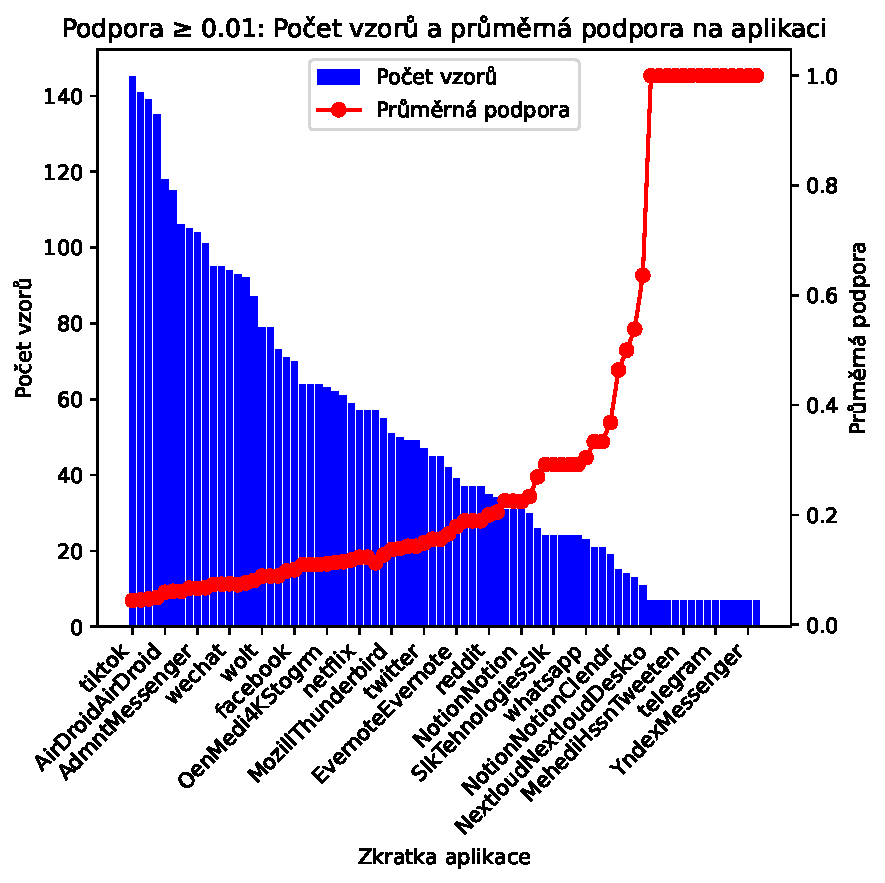
\includegraphics[width=\linewidth]{obrazky-figures/exps/patterns_support_0.01_mobile.pdf}
		\caption{Počet vzorů a~průměrná podpora na~aplikaci -- \texttt{mobile desktop apps.csv}}
		\label{fig:graph-num-vs-apps-mobile-001}
	\end{minipage}
	\hfill
	\begin{minipage}[t]{0.49\textwidth}
		\centering
		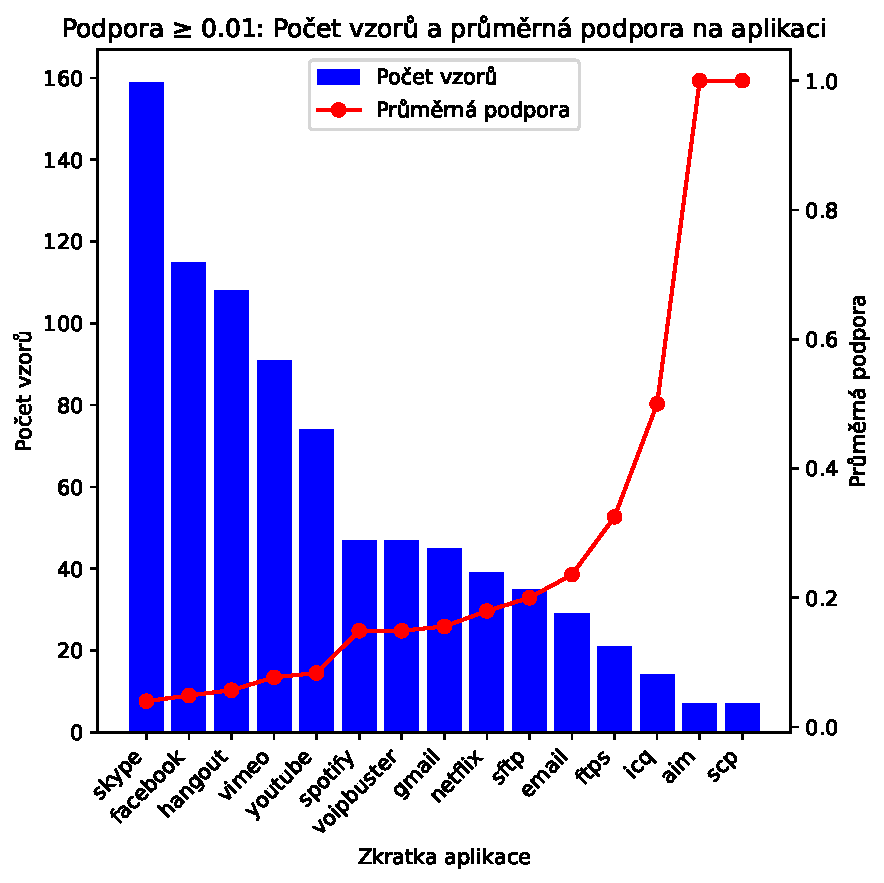
\includegraphics[width=\linewidth]{obrazky-figures/exps/patterns_support_0.01_iscx.pdf}
		\caption{Počet vzorů a~jejich průměrná podpora na~aplikaci -- \texttt{iscx.csv}}
		\label{fig:graph-num-vs-apps-iscx-001}
	\end{minipage}
\end{figure}


Graf na~obrázku\footnote{U všech následujících grafů jsou z~důvodu přehlednosti zobrazeny popisky pouze pro~každou čtvrtou aplikaci z~datové sady \texttt{mobile\_desktop\_apps\_raw.csv}.}~\ref{fig:graph-num-vs-apps-mobile-001} znázorňuje počet získaných vzorů při~prahu minimální podpory 0{,}01 pro~každou aplikaci z~datové sady \texttt{mobile\_desktop\_apps\_raw.csv}. Je patrné, že mezi~aplikací s~nejnižším a~nejvyšším počtem vzorů je výrazný rozdíl — konkrétně až \textbf{130 vzorů}. V~grafu je rovněž vyznačena průměrná podpora vytěžených vzorů pro~jednotlivé aplikace, přičemž lze pozorovat, že některé aplikace obsahují vzory s~podporou rovnou 1{,}0. To znamená, že se tyto vzory vyskytují ve všech jejich instancích. Tento jev lze pravděpodobně přičíst malému testovacímu vzorku daných aplikací.

Obdobně je v~grafu na~obrázku~\ref{fig:graph-num-vs-apps-iscx-001} znázorněn průměrný počet vzorů a~jejich podpora pro~jednotlivé aplikace v~datové sadě \texttt{iscx.csv}. Také v~tomto případě je patrný výrazný rozdíl v~počtu vzorů mezi~jednotlivými aplikacemi, který dosahuje až \textbf{152 vzorů}. Kompletní přehled, počtu vzorů a~jejich průměrné podpory pro~dříve zmíněné hodnoty minimální podpory, je uveden v Příloze~\ref{sec:appendix:ex2}.

Kvůli tomuto výraznému nepoměru v~počtu vzorů napříč aplikacemi bylo nutné při~výpočtu podobnosti zohlednit nejen samotnou přítomnost vzorů, ale i~jejich podporu (frekvenci výskytu v~rámci dané aplikace) a~unikátnost (míru výskytu napříč všemi aplikacemi), jak je popsáno v~podsekci~\ref{subsec:klicove}. 

Alternativním přístupem je normalizace počtu vzorů mezi~aplikacemi, například filtrováním na~přibližně stejný počet vzorů podle stanovených kritérií (např. délka či podpora). Tento krok by mohl předejít zkreslení, které vzniká v~případech, kdy některé aplikace disponují nepřiměřeně vysokým počtem vzorů s~nízkou podporou, zatímco jiné obsahují pouze několik málo specifických a~silně reprezentativních vzorů. Při~vyšší minimální podpoře již není rozdíl v~počtu získaných vzorů mezi~aplikacemi tak markantní. Nicméně identifikace při~stejném počtu informativně rovnocenných vzorů by měla teoreticky být vyváženější a~tím pádem přesnější.

Z tohoto důvodu je provedena analýza délky vzorů pro~jednotlivé aplikace. Kratší vzory mají tendenci vést k~častějším, ale obecnějším identifikacím, zatímco delší vzory mohou poskytnout specifičtější identifikaci, avšak s~nižší frekvencí výskytu.

\begin{figure}[H]
	\centering
	\begin{minipage}[t]{0.5\textwidth}
		\centering
		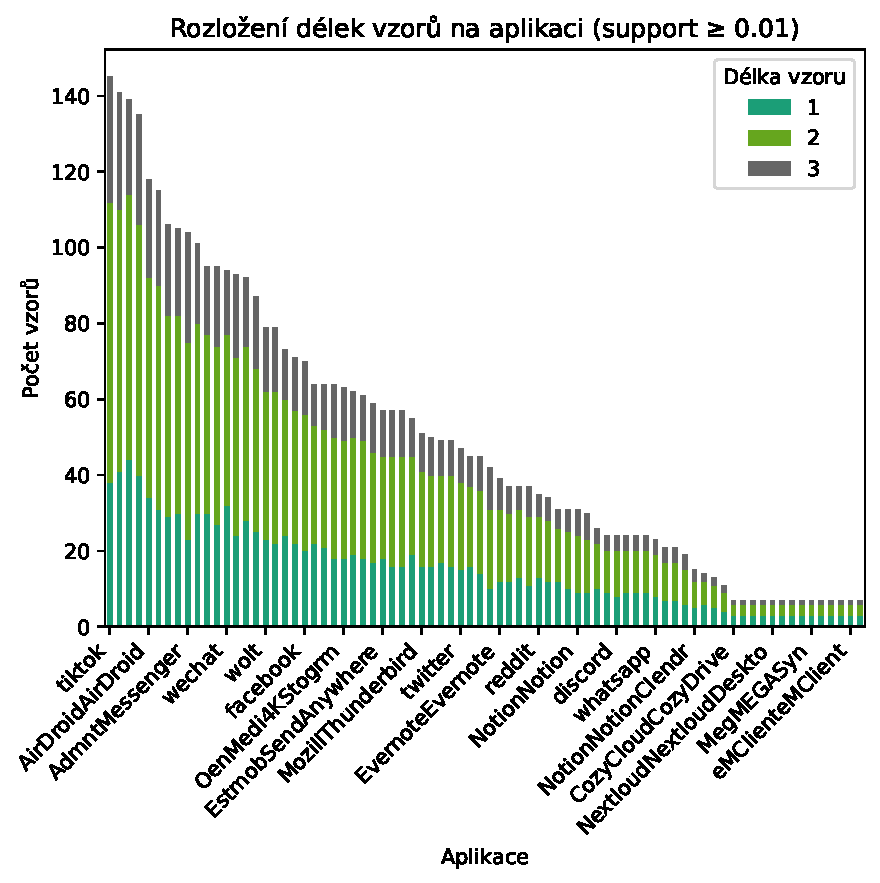
\includegraphics[width=\linewidth]{obrazky-figures/exps/pattern_lengths_0.01_mobile.pdf}
		\caption{Rozložení délek vzorů na~aplikaci při~minimální podpoře 0{,}01 pro~\texttt{mobile desktop apps raw.csv}}
		\label{fig:ex2-mobile-patterns-len}
	\end{minipage}
	\hfill
	\begin{minipage}[t]{0.49\textwidth}
		\centering
		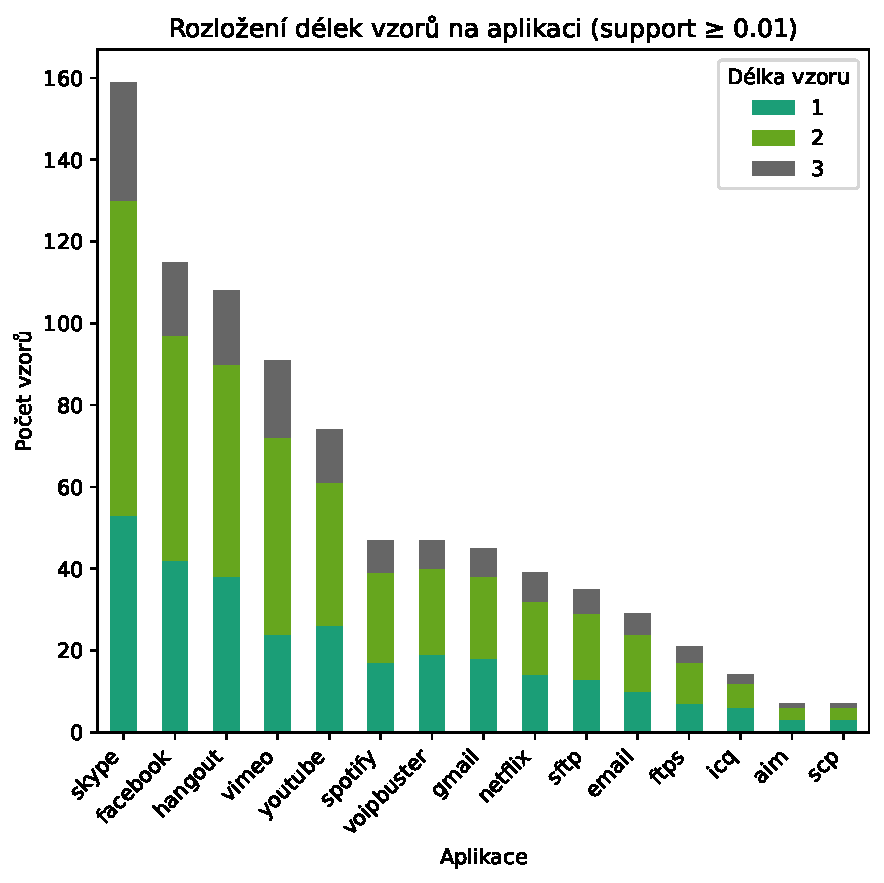
\includegraphics[width=\linewidth]{obrazky-figures/exps/pattern_lengths_0.01_iscx.pdf}
		\caption{Rozložení délek vzorů na~aplikaci při~minimální podpoře 0{,}01 pro~\texttt{iscx.csv}}
		\label{fig:ex2-iscx-patterns-len}
	\end{minipage}
\end{figure}

Grafy na~obrázcích~\ref{fig:ex2-mobile-patterns-len} a~\ref{fig:ex2-iscx-patterns-len} znázorňují rozložení délek získaných vzorů aplikací při~minimální podpoře 0.01 pro~datové sady \texttt{mobile\_desktop\_apps\_raw.csv} a~\texttt{iscx.csv}. V~obou případech převažují vzory o~délce 1 a~2. Jak bylo již uvedeno, vzory o~délce 3 jsou méně časté, ale mohou poskytnout informativně cennější hodnotu díky své specifičnosti. 

Viz.grafy na~obrázcích~\ref{fig:ex2-mobile-patterns-len-025} a~\ref{fig:ex2-iscx-patterns-len-025}, které znázorňují stejnou závislost při~změně hodnoty minimální podpory, která je nyní nastavena na~0.25. Při~této podpoře jsou častější obecnější vzory o~délce 1, zatímco vzory o~délce 3 jsou zde zastoupeny ve výrazně menším počtu, v~některých případech již vůbec. Hodnota podpory 0.26 představuje hranici pro~oba datové soubory. Při~této hodnotě již pro~některé aplikace nebyly nalezeny žádné vzory. Konkrétně se jedná o~aplikaci \textit{facebook} v~datové sadě \texttt{iscx.csv} a~\textit{alipay} v~sadě \texttt{mobile\_desktop\_apps\_raw.csv}. Tento jev je patrný i~v~grafech, kde je zřetelný pokles počtu vzorů, přičemž u~těchto aplikací, jako je \textit{facebook} a~\textit{alipay}, se v~tomto rozmezí nachází pouze jeden vzor.

\begin{figure}[H]
	\centering
	\begin{minipage}[t]{0.5\textwidth}
		\centering
		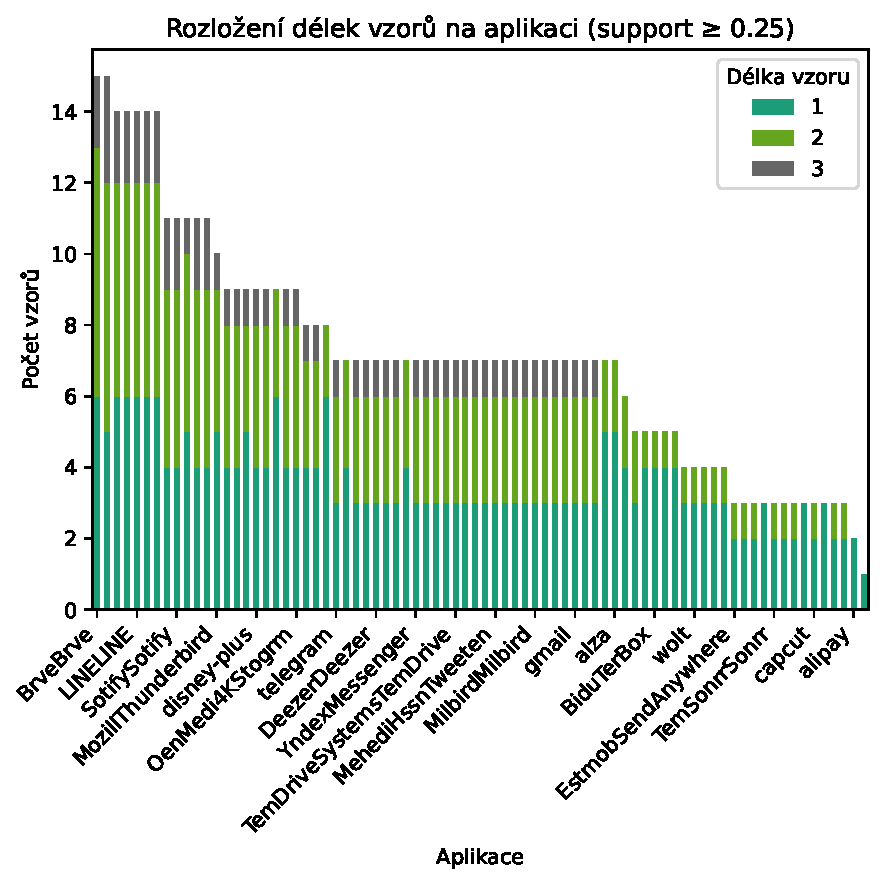
\includegraphics[width=\linewidth]{obrazky-figures/exps/pattern_lengths_0.25_mobile.pdf}
		\caption{Rozložení délek vzorů na~aplikaci při~minimální podpoře 0{,}25 pro~\texttt{mobile desktop apps raw.csv}}
		\label{fig:ex2-mobile-patterns-len-025}
	\end{minipage}
	\hfill
	\begin{minipage}[t]{0.49\textwidth}
		\centering
		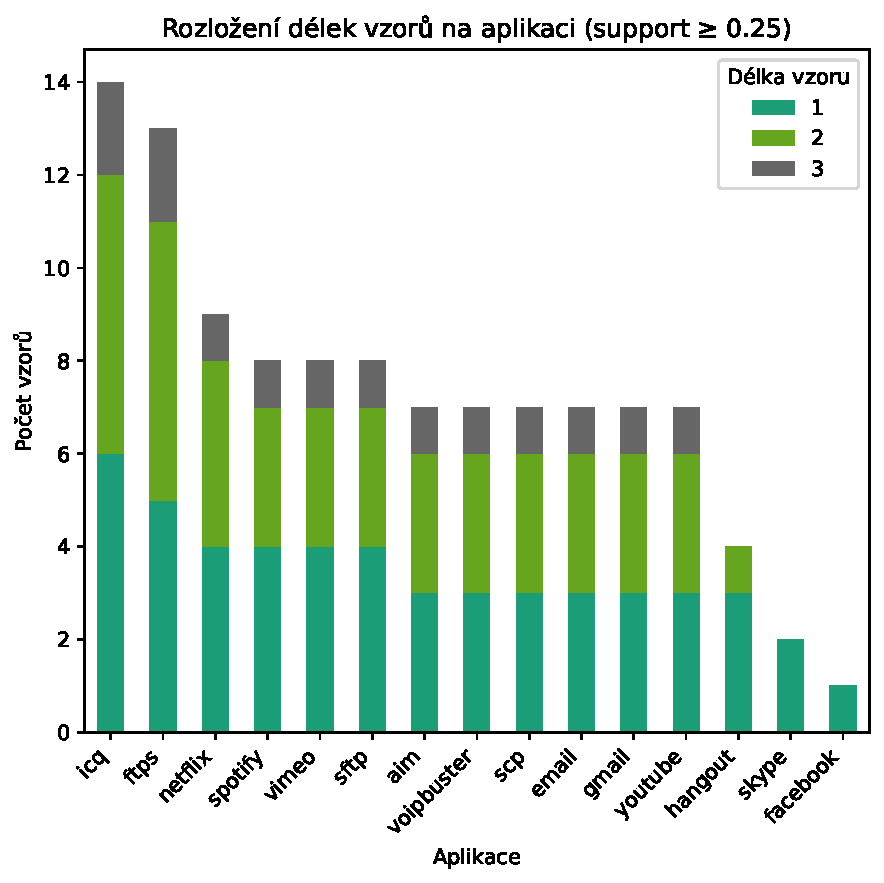
\includegraphics[width=\linewidth]{obrazky-figures/exps/pattern_lengths_0.25_iscx.pdf}
		\caption{Rozložení délek vzorů na~aplikaci při~minimální podpoře 0{,}25 pro~\texttt{iscx.csv}}
		\label{fig:ex2-iscx-patterns-len-025}
	\end{minipage}
\end{figure}

Vzory byly filtrovány dle délky, přičemž v~rámci každé délkové skupiny byly seřazeny podle podpory. Byla vytvořena sada filtrů na~základě předchozí analýzy počtu a~délky vzorů. Následně bylo z~každé množiny vybráno $N$ vzorů podle zvoleného filtru.

Různé varianty filtrů byly otestovány pro~čtyři hodnoty minimální podpory: \textbf{0{,}01}, \textbf{0{,}05}, \textbf{0{,}2} a~\textbf{0{,}25}. Jako vstupní množina pro~algoritmus \textit{Apriori} byly konzistentně použity otisky \textit{JA4}, \textit{JA4S} a~atribut spojení \textit{SNI}. Cílem této fáze bylo porovnat přesnost výsledné kandidátní množiny vůči referenčnímu stavu bez~jakékoli filtrace (viz~Obrázky~\ref{fig:ex2-iscx-heatmap} a~\ref{fig:ex2-mobile-heatmap}).

Následující tabulky shrnují nejzajímavější výsledky jednotlivých filtrů z~hlediska identifikační přesnosti a~počtu použitých vzorů. \textbf{Kombinace} označují konkrétní otisky a~atributy spojení použitých pro~generování počáteční kandidátní množiny. \textbf{Podpora} udává hodnotu minimální podpory použitou při~těžbě vzorů. \textbf{Filtr} reprezentuje způsob filtrování vzorů ve formátu \(len(n)Xm\), kde \(len(n)\) označuje délku vzoru a~\(Xm\) specifikuje počet takových vzorů. Pokud je parametr \(Xm\) vynechán, znamená to, že jsou použity všechny vzory dané délky. Dále byly testovány i~kombinace více filtrů, které jsou označeny symbolem \(+\). 

\begin{table}[H]
	\centering
	\begin{tabular}{lrlll}
		\toprule
		\multicolumn{5}{c}{\texttt{iscx.csv}}  \\
		\midrule
		Kombinace    & Podpora & Filtr              & Přesnost & Prům. délka množiny \\
		\midrule
		JA4          & 0.01    & len(1)x5+len(3)x10 & 0.91      & 2.128395                    \\
		JA4          & 0.01    & len(2)x5           & 0.91      & 2.128395                    \\
		JA4          & 0.01    & len(3)             & 0.91      & 2.128395                    \\
		JA4+JA4S+SNI & 0.05    & len(3)x10          & 0.89      & 1.585185                    \\
		JA4+JA4S+SNI & 0.05    & len(3)             & 0.89      & 1.585185                    \\
		JA4+JA4S+SNI & 0.05    & len(3)x5           & 0.89      & 1.585185                    \\
		\bottomrule
	\end{tabular}
	\caption{Top 3 výsledky, pro~každou kombinaci generující počáteční množinu,  podle přesnosti s~aplikací filtrů  u~datové sady \texttt{iscx.csv}}
	\label{tab:top3-iscx}
\end{table}

V tabulce~\ref{tab:top3-iscx} jsou uvedeny výsledky přesnosti jednotlivých filtrů pro~datovou sadu \texttt{iscx.csv}. Kombinace \textit{JA4}, která vytváří počáteční množinu, vykazuje velmi mírné zlepšení u~výše zmíněných filtrů, přičemž průměrná velikost kandidátní množiny zůstává nezměněna. Druhá kombinace \textit{JA4+JA4S+SNI} nevykazuje žádné zlepšení.

\begin{table}[H]
	\centering
	\begin{tabular}{lrlll}
		\toprule
		\multicolumn{5}{c}{\texttt{mobile\_desktop\_apps\_raw.csv}}  \\
		\midrule
		Kombinace    & Podpora & Filtr              & Přesnost & Prům. délka množiny \\
		\midrule
		JA4+JA4S+SNI & 0.01    & len(1)x2+len(3)x2  & 0.81      & 1.713638                    \\
		JA4+JA4S+SNI & 0.05    & len(1)x2+len(3)x2  & 0.81      & 1.713638                    \\
		JA4+JA4S+SNI & 0.20    & len(1)x5+len(2)x10 & 0.81      & 1.713638                    \\
		JA4          & 0.01    & len(2)x5+len(3)x10 & 0.80      & 2.790678                    \\
		JA4          & 0.01    & len(2)x5+len(3)x5  & 0.78      & 2.790678                    \\
		JA4          & 0.01    & len(3)             & 0.78      & 2.790678                    \\
		\bottomrule
	\end{tabular}
	\caption{Top 3 výsledky, pro~každou kombinaci generující počáteční množinu,  podle přesnosti s~aplikací filtrů  u~datové sady \texttt{mobile desktop apps raw.csv}}
	\label{tab:top3-mobile}
\end{table} 

Datová sada \texttt{mobile\_desktop\_apps\_raw.csv} při~použití filtrů taktéž nevykazuje žádné významné zlepšení v~přesnosti identifikace ani ve zmenšení velikosti kandidátní množiny (viz. Tabulka~\ref{tab:top3-mobile}). Přestože se mohou výsledky jevit jako málo přínosné, z~pohledu optimalizace procesu identifikace přinášejí určitý benefit -- zejména v~podobě redukce počtu vzorů, které je nutné porovnávat, a~jejich částečné normalizace napříč aplikacemi.

Z tabulek~\ref{tab:top3-mobile} a~\ref{tab:top3-iscx} je patrné, že nejlepších výsledků přesnosti je dosahováno při~různých kombinacích filtrů a~parametrů pro~každou z~datových sad. Zatímco pro~\texttt{iscx.csv} se jako nejefektivnější jeví selekce zaměřená na~delší vzory (např. \texttt{len(3)} nebo \texttt{len(2)x5}) a~nižší hodnoty podpory, u~datové sady \texttt{mobile\_desktop\_apps\_raw.csv} dosahují srovnatelné přesnosti filtry kombinující obecné a~specifické vzory (např. \texttt{len(1)x2+len(3)x2}) i~při~vyšších hodnotách podpory.

Použitím nižší hodnoty minimální podpory je zároveň možné zachytit i~méně časté, ale informačně hodnotnější vzory. Ty mohou být klíčové pro~přesnější rozlišení mezi~jednotlivými spojeními, která nelze efektivně identifikovat pomocí obecnějších vzorů vznikajících při~vyšších prahových hodnotách. Aplikace filtrů pak umožňuje tyto specifické vzory v~databázi ponechat, čímž přispívá k~vyváženějšímu kompromisu mezi~výpočetní efektivitou a~identifikační schopností.

\begin{wrapfigure}{r}{0.5\textwidth}
	\centering
	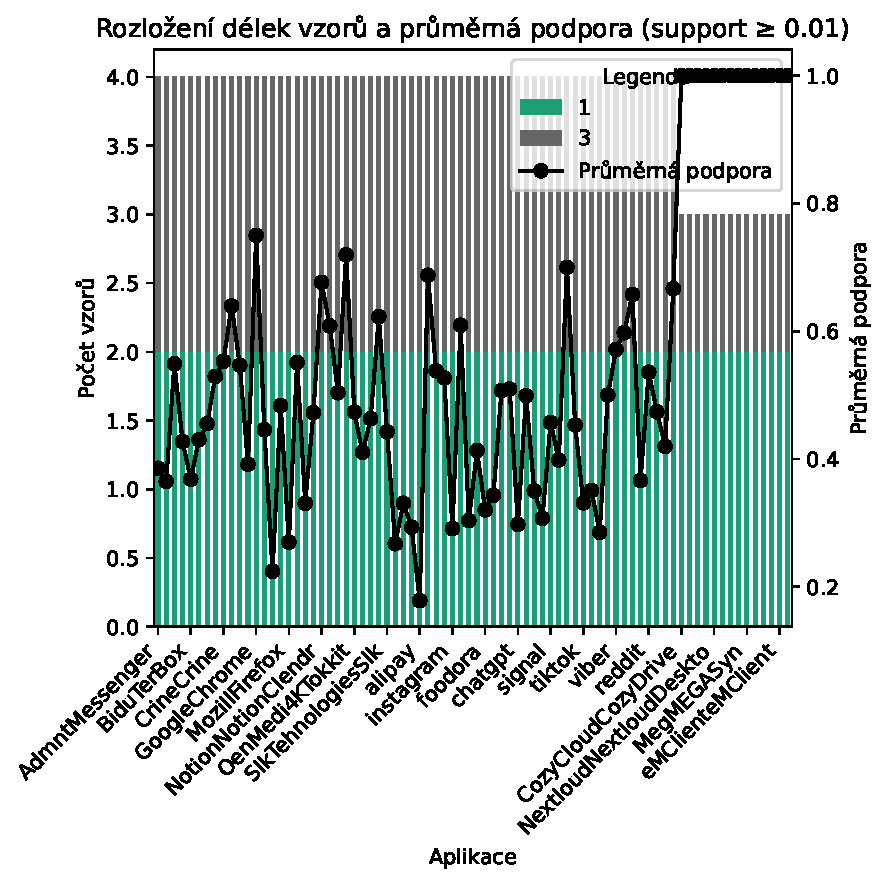
\includegraphics[width=0.49\textwidth]{obrazky-figures/exps/pattern_lengths_filtered_0.01_mobile.pdf}
	\caption{Rozložení délek vzorů a~průměrná podpora po~aplikaci filtrace \texttt{len(1)x2 a~len(3)x2} pro~\texttt{mobile desktop apps raw.csv} s~minimální podporou 0{,}01}
	\label{fig:pattern_lengths-filtered-mobile}
\end{wrapfigure}

Graf na~obrázku~\ref{fig:pattern_lengths-filtered-mobile} znázorňuje aplikovanou selekci pomocí filtru \texttt{len(1)x2 + len(3)x2} a~minimální podpory \textbf{0{,}01} pro~datovou sadu \texttt{mobile\_desktop\_apps\_raw.csv}. Toto nastavení dosahuje přesnosti \textbf{0{,}8129} při~průměrné velikosti finální kandidátní množiny \textbf{1{,}7}. Modus i~medián této velikosti jsou rovny \textbf{1}. Většina aplikací si uchovává právě dva vzory délky 1 a~dva vzory délky 3. U~menšiny aplikací však nebyly nalezeny dva vzory délky 3, ale pouze jeden.

Tento experiment ukázal, že selektivní filtrování vzorů může vést k~efektivnější (méně náročnější) identifikaci, přičemž negativní dopad na~přesnost se projevuje až při~použití vyšších hodnot minimální podpory. Při~nízké podpoře a~vhodně zvolených filtrech je tento dopad téměř zanedbatelný (viz~\ref{sec:appendix:ex2}). 

Přestože se nejedná o~univerzálně aplikovatelné řešení, výsledky potvrzují, že pro~různé datové sady je možné nalézt vhodnou kombinaci parametrů (podpora, délka, počet vzorů), která zajistí optimální rovnováhu mezi~výpočetní náročností a~kvalitou identifikace. Kompletní výsledky se všemi použitými filtry pro~obě datové sady a~obě kombinace jsou uvedeny v~příloze~\ref{chp:appendix-experiments}.

\section{Šířka okna určující okolí spojení}
\label{sec:ex-window}
Kontext každého identifikovaného spojení je určen velikostí posuvného okna, jak je popsáno v~podsekci~\ref{subsec:klicove}. Ve většině případů se ve středu tohoto okna nachází právě identifikované spojení, zatímco jeho okolí může tvořit buď další spojení stejné aplikace (například v~rámci jednoho spuštění), nebo spojení patřící jiným aplikacím. Vzhledem k~náhodnému uspořádání testovací množiny může dojít k~tomu, že do~okna spadají i~nesouvisející spojení, což způsobuje informační šum a~může negativně ovlivnit kvalitu identifikace.

Cílem tohoto experimentu je určit optimální velikost okna, která zachytí dostatek relevantního kontextu pro~přesnou identifikaci, aniž by zahrnovala rušivá data z~jiných aplikací. 

V~rámci experimentu byly parametry nastaveny na~použití metody \textbf{\textit{JA4+JA4S+SNI}} jak pro~generování \textbf{počáteční} kandidátní množiny, tak i~pro~nalezení \textbf{častých vzorů}. \textbf{Minimální podpora} byla nastavena na~\textbf{0{,}01} a~byla využita selekce filtrů z~předchozího experimentu. Maximální počet kandidátů byl zvolen na~\textbf{3}. Testovány byly různé hodnoty šířky kontextového okna (vždy liché číslo, aby byl kontext z~obou stran vyvážen), konkrétně \textbf{3, 5, 7, 9, 11, 21} a~\textbf{31}.
V~tabulce~\ref{tab:used_filters-ex4} jsou uvedeny jednotlivé použité filtry, které byly zvoleny na~základě nejvyšší dosažené přesnosti v~předchozím experimentu.

\begin{table}[H]
	\centering
	\begin{tabular}{lll}
		\toprule
		Kombinace    & \texttt{mobile\_desktop\_apps\_raw.csv} & \texttt{iscx.csv}  \\
		\midrule
		JA4          & len(2)x5+len(3)x10                      & len(1)x5+len(3)x10 \\
		JA4+JA4S+SNI & len(1)x2+len(3)x2                       & len(3)x5           \\
		\bottomrule
	\end{tabular}
	\caption{Použité filtry pro~experiment}
	\label{tab:used_filters-ex4}
\end{table}
Následující tabulky uvádějí použitou šířku okna a~přesnost pro~daný otisk nebo kombinaci otisků, které byly použity pro~generování počáteční množiny. Nejvyšší dosažené přesnosti jsou v~tabulkách vyznačeny tučně.

\begin{table}[H]
	\centering
	\begin{minipage}{0.49\textwidth}
		\centering
		\begin{tabular}{cll}
			\toprule
			\multicolumn{3}{c}{\texttt{mobile\_desktop\_apps\_raw.csv}}  \\
			\midrule
			\multirow{2}{*}{Šířka okna} & \multicolumn{2}{l}{Přesnost při~kombinacích}\\
															    			
			            & JA4             & JA4+JA4S+SNI    \\
			\midrule
			\textbf{3}  & 0.7706          & \textbf{0.8157} \\
			5           & 0.8058          & 0.8133          \\
			7           & 0.8289          & 0.8133          \\
			\textbf{9}  & \textbf{0.8332} & 0.8131          \\
			\textbf{11} & 0.8280          & \textbf{0.8157} \\
			21          & 0.7644          & 0.8013          \\
			31          & 0.6877          & 0.7874          \\
			\bottomrule
		\end{tabular}
		\caption{Přesnost identifikace pro~různé velikosti okolí pro~datovou sadu \texttt{mobile desktop apps raw.csv}.}
		\label{tab:mobile_acc_vs_window}
										        
	\end{minipage}
	\hfill
	\begin{minipage}{0.49\textwidth}
												
		\centering
		\begin{tabular}{cll}
			\toprule
			\multicolumn{3}{c}{\texttt{iscx.csv}}  \\
			\midrule
			\multirow{2}{*}{Šířka okna} & \multicolumn{2}{l}{Přesnost při~kombinacích}\\
																		
			            & JA4             & JA4+JA4S+SNI    \\
			\midrule
			3           & 0.9111          & 0.8815          \\
			5           & 0.9012          & 0.8840          \\
			7           & 0.9012          & 0.8864          \\
			9           & 0.9062          & 0.8864          \\
			\textbf{11} & 0.9062          & \textbf{0.8914} \\
			\textbf{21} & \textbf{0.9185} & 0.8840          \\
			31          & 0.8864          & 0.8691          \\
			\bottomrule
		\end{tabular}
		\caption{Přesnost identifikace pro~různé velikosti okolí s~\textit{JA4+JA4S+SNI} a~\textit{JA4} pro~datovou sadu \texttt{iscx.csv}.}
		\label{tab:iscx_acc_vs_window}
										        
	\end{minipage}
\end{table}

Na základě analýzy bylo zjištěno, že optimální šířka okna pro~jednotlivé datové sady se částečně odvíjí od~průměrného počtu spojení při~jednom spuštění aplikace. U~sady \texttt{mobile\_desktop\_apps\_raw.csv}, kde je průměrný \textbf{počet spojení 3{,}15 na~jedno spuštění aplikace}, byly nejlepší výsledky dosaženy při~\textbf{menší šířce} okna 9 nebo 11 (viz.~Tabulka~\ref{tab:mobile_acc_vs_window}). Naproti tomu u~sady \texttt{iscx.csv}, kde je průměrný \textbf{počet spojení v~rámci jednoho spuštění vyšší a~to 4{,}55}, se optimální přesnost posunula k~\textbf{širším oknům 11 a~21} (viz.~Tabulka~\ref{tab:iscx_acc_vs_window}). I~velmi úzké \textbf{okno o~velikosti 3} přináší konkurenceschopné výsledky, což lépe odpovídá průměrnému počtu spojení v~jednotlivých spuštěních aplikací v~testovací množině.

Vzhledem k~tomu, že testovací množina byla sestavena tak, že obsahuje přibližně 25~\% spojení z~každého spuštění (viz.podsekce~\ref{subsec:klicove}), může nedostatek širšího kontextu v~testovacích datech negativně ovlivnit konečné výsledky klasifikace. Chybějící návaznosti mezi~spojeními mohou omezit schopnost zachytit frekventované vzory, které by při~plnějším kontextu mohly být lépe rozpoznatelné.

Je však třeba poznamenat, že ve skutečném síťovém provozu zpravidla nebývá možné zachytit čistě oddělená spuštění jednotlivých aplikací bez~jakéhokoli informačního šumu pocházejícího od~jiných procesů. Volba strategie, kdy je testovací množina sestavena pouze ze zlomku spojení napříč jednotlivými spuštěními, tak do~určité míry simuluje reálnou situaci, kdy je třeba aplikace identifikovat v~prostředí s~překrývající se či souběžně probíhající komunikací. V~budoucnu by bylo možné zkoumat například vliv typu aplikace na~ideální šířku okna, nebo adaptivní strategie, které dynamicky upravují velikost okna podle délky nebo hustoty síťové komunikace dané aplikace.


\section{Volba maximálního počtu kandidátů a~její vliv na~přesnost identifikace}
Posledním parametrem, který přímo ovlivňuje přesnost identifikace a~délku finální kandidátní množiny, je maximální počet kandidátů -- tedy výsledná maximální délka finální množiny kandidátů. Experiment zaměřený na~volbu tohoto parametru se soustředí na~finální přesnost identifikace a~její porovnání s~výsledky fingerprintingu pomocí metod \textit{JA4} a~\textit{JA4+JA4S+SNI}. Počáteční kandidátní množina je v~rámci experimentu určena jak metodou \textbf{\textit{JA4}}, tak metodou \textbf{\textit{JA4+JA4S+SNI}}. Vstupem pro~\textit{Apriori} jsou položky \textbf{\textit{JA4}}, \textbf{\textit{JA4S}} a~\textbf{\textit{SNI}}. Šířka okna určující kontext spojení byla nastavena na~\textbf{3 spojení}, jelikož experiment popsaný v~sekci~\ref{sec:ex-window} ukazuje na~tuto šířku jako na~univerzální pro~obě datové sady i~obě testované kombinace. Testování identifikace proběhlo \textbf{s minimální podporou 0.01 a~0.2} pro~soubor \texttt{mobile\_desktop\_apps\_raw.csv} a~\textbf{0.01 a~0.25} pro~soubor \texttt{iscx.csv}. Tyto hodnoty se ukázaly jako ideální v~předchozím experimentu popsaném v~sekci~\ref{ex-min_sup}. Pro~práh podpory 0.01 při~těžbě jsou uvedeny dvě verze výsledků -- \textbf{s filtrem} (každý filtr byl zvolen shodně jako v~předchozím experimentu v~sekci~\ref{sec:ex-window}) \textbf{a bez~filtru}. Maximální zkoumaný počet kandidátů je \textbf{4} pro~\texttt{iscx.csv} a~\textbf{9} pro~\texttt{mobile\_desktop\_apps\_raw.csv}. Časové hodnoty byly měřeny na~testovacím zařízení s~následujícími parametry: CPU: \texttt{AMD Ryzen 7 5700U (16) @ 1.80 GHz}, OS:\texttt{ EndeavourOS x86\_64}, RAM: \texttt{16 GB}.

\subsection{Výsledky pro~\texttt{iscx.csv}}
V této sekci se budou experimenty zabývat pouze datovou sadou \texttt{iscx.csv}.
\begin{table}[H]
	\centering
	\begin{tabular}{lcc}
		\toprule
		\multicolumn{3}{c}{\texttt{iscx.csv}} \\
		\midrule
		          & \textbf{JA4} & \textbf{JA4+JA4S+SNI} \\
		\midrule
		Přesnost & 0.975        & 0.924                 \\
		Délka    & 3.146        & 2.094                 \\
		\bottomrule
	\end{tabular}
	\caption{Přesnost fingerprintingu \textit{JA4} a~jejich kombinace pro~\texttt{iscx.csv}}
	\label{tab:iscx-fingerprints-accuracy}
\end{table} 

Tabulka~\ref{tab:iscx-fingerprints-accuracy} uvádí přesnost a~průměrnou délku kandidátní množiny po~aplikaci otisků \textit{JA4} a~\textit{JA4+JA4S+SNI} (bez využiti kontextu). Na~tuto tabulku bude dále odkazováno při~porovnání jednotlivých verzí v~rámci testování.


\begin{table}[H]
	\centering
	\begin{tabular}{c|rrr|rrr}
		\toprule
		\multicolumn{7}{c}{\texttt{iscx.csv} s~minimální podporou 0{,}01}  \\
		\midrule
		\multirow{2}{*}{Počet kandidátů} & \multicolumn{3}{c}{JA4} & \multicolumn{3}{c}{JA4+JA4S+SNI}\\
		  & Přesnost & Čas [s] & Prům. délka & Přesnost & Čas [s] & Prům. délka \\
		\midrule
		1 & 0.635     & 16.567   & 1.000         & 0.679     & 16.567   & 1.000         \\
		2 & 0.827     & 13.919   & 1.649         & 0.832     & 13.919   & 1.385         \\
		3 & 0.899     & 16.752   & 2.128         & 0.874     & 16.752   & 1.585         \\
		4 & 0.951     & 16.847   & 2.454         & 0.923     & 16.847   & 1.751         \\
		\bottomrule
	\end{tabular}
	\caption{Výsledky experimentu s~různým nastavením maximálního počtu kandidátů při~minimální podpoře 0{,}01, porovnávající metody \textit{JA4} a~\textit{JA4+JA4S+SNI} pro~generování počáteční kandidátní množiny nad~datovou sadou \texttt{iscx.csv}.}
	\label{tab:iscx_sup_01}
\end{table}

Při minimální podpoře 0{,}01 bez~použití filtrů (viz.Tabulka~\ref{tab:iscx_sup_01}) dosahuje jednoznačná identifikace úspěšnosti mezi~63{,}5~\% a~67{,}8~\%. Při~maximálním počtu kandidátů rovném 4 je přesnost identifikace založená pouze na~otisku \textit{JA4} o~\textbf{2{,}4~\%} nižší, nicméně průměrná velikost finální kandidátní množiny je menší -- \textbf{2{,}5} oproti \textbf{3{,}1}. Při~využití kombinace \textit{JA4+JA4S+SNI} je přesnost \textbf{téměř identická}, avšak velikost kandidátní množiny se snižuje na~\textbf{1{,}75 oproti 2{,}094}. Celková doba trvání identifikace se pohybuje v~rozmezí \textbf{13 až 17} sekund.

\begin{table}[H]
	\centering
	\begin{tabular}{c|rrr|rrr}
		\toprule
		\multicolumn{7}{c}{\texttt{iscx.csv} s~minimální podporou 0{,}25}  \\
		\midrule
		\multirow{2}{*}{Počet kandidátů} & \multicolumn{3}{c}{JA4} & \multicolumn{3}{c}{JA4+JA4S+SNI}\\
		  & Přesnost & Čas [s] & Prům. délka & Přesnost & Čas [s] & Prům. délka \\
		\midrule
		1 & 0.607     & 1.370    & 1.000         & 0.751     & 1.370    & 1.000         \\
		2 & 0.701     & 1.385    & 1.649         & 0.817     & 1.385    & 1.385         \\
		3 & 0.859     & 1.480    & 2.128         & 0.872     & 1.480    & 1.585         \\
		4 & 0.904     & 1.861    & 2.454         & 0.881     & 1.861    & 1.751         \\
		\bottomrule
	\end{tabular}
	\caption{Výsledky experimentu s~různým nastavením maximálního počtu kandidátů při~minimální podpoře 0{,}25, porovnávající metody \textit{JA4} a~\textit{JA4+JA4S+SNI} pro~generování počáteční kandidátní množiny nad~datovou sadou \texttt{iscx.csv}.}
	\label{tab:iscx_sup_25}
\end{table}

V případě vyšší minimální podpory, jak je uvedeno v~Tabulce~\ref{tab:iscx_sup_25}, klesá doba trvání identifikace na~pouhých \textbf{1{,}3 až 1{,}8 sekundy}. Jednoznačná identifikace s~použitím kombinace otisků dosahuje vyšší úspěšnosti. Při~použití maximálně čtyř kandidátů vykazuje metoda \textit{JA4} \textbf{ztrátu 7{,}1\%}, zatímco kombinace ztrácí pouze \textbf{3{,}3~\%}. Průměrná délka finální kandidátní množiny zůstává nezměněna, což je dáno jejím omezením maximálním počtem kandidátů.

Ideálním kompromisem se jeví použití minimální podpory \textbf{0,01 s~aplikací filtrů} (viz. Tabulka~\ref{tab:iscx_sup_01_filters}). Metoda \textit{JA4} vykazuje ztrátu\textbf{ 4{,}4\%} v~přesnosti, přičemž doba trvání identifikace se pohybuje mezi~\textbf{2 až 3} sekundami. Kombinace \textit{JA4+JA4S+SNI} ztrácí méně, konkrétně \textbf{2\%}, a~zároveň je \textbf{nejrychlejší} z~testovaných verzí, s~dobou trvání kolem \textbf{1{,}1 až 1{,}2 sekundy}.
\begin{table}[H]
	\centering
	\begin{tabular}{c|rrr|rrr}
		\toprule
		\multicolumn{7}{c}{\texttt{iscx.csv} s~minimální podporou 0{,}01 s~filtry}  \\
		\midrule
		\multirow{2}{*}{Počet kandidátů} & \multicolumn{3}{c}{JA4} & \multicolumn{3}{c}{JA4+JA4S+SNI}\\
		  & Přesnost & Čas [s] & Prům. délka & Přesnost & Čas [s] & Prům. délka \\
		\midrule
		1 & 0.647     & 2.100    & 1.000         & 0.664     & 1.168    & 1.000         \\
		2 & 0.847     & 3.576    & 1.649         & 0.805     & 1.146    & 1.385         \\
		3 & 0.906     & 2.217    & 2.128         & 0.881     & 1.191    & 1.585         \\
		4 & \textbf{0.931}     & \textbf{2.355}    & \textbf{2.454}         & \textbf{0.904}     & \textbf{1.281}    & \textbf{1.751}         \\
		\bottomrule
	\end{tabular}
	\caption{Výsledky experimentu s~různým nastavením maximálního počtu kandidátů při~minimální podpoře \textbf{0{,}25}, porovnávající metody \textit{JA4} a~\textit{JA4+JA4S+SNI} pro~generování počáteční kandidátní množiny a~aplikaci selekce vzorů pomocí filtrů nad~datovou sadou \texttt{iscx.csv}. Aplikovaný filtr pro~\textit{JA4} \texttt{len(1)x5+len(3)x10}, zatímco pro~kombinaci \textit{JA4+JA4S+SNI} byl zvolen filtr \texttt{len(3)x5}.}
	\label{tab:iscx_sup_01_filters}
\end{table}


\subsection{Výsledky pro~\texttt{mobile\_desktop\_apps\_raw.csv}}
V této sekci se budou experimenty zabývat pouze datovou sadou \texttt{mobile\_desktop\_apps\_raw}.
\begin{table}[H]
	\centering
	\begin{tabular}{lcc}
		\toprule
		\multicolumn{3}{c}{\texttt{mobile\_desktop\_apps\_raw.csv}} \\
		\midrule
		          & \textbf{JA4} & \textbf{JA4+JA4S+SNI} \\
		\midrule
		Přesnost & 0.966        & 0.854                 \\
		Délka    & 14.298       & 3.382                 \\
		\bottomrule
	\end{tabular}
	\caption{Přesnost otisků \textit{JA4} a~jejich kombinací pro~\texttt{mobile desktop apps raw.csv}}
	\label{tab:mobile-fingerprints-accuracy}
\end{table} 

Tabulka~\ref{tab:mobile-fingerprints-accuracy} uvádí přesnost a~průměrnou délku kandidátní množiny po~aplikaci otisků \textit{JA4} a~\textit{JA4+JA4S+SNI} (bez kontextu). Na~tuto tabulku bude dále odkazováno při~porovnání jednotlivých verzí v~rámci testování.

Vysoká přesnost identifikace by mohla být očekávána u~následující varianty (minimální podpora 0{,}01 bez~filtrování vzorů), avšak dosažené výsledky naznačují opak (viz.~\ref{tab:mobile-001}). U~metody \textit{JA4} dochází při~maximálním počtu kandidátů, tedy 9, k~poklesu přesnosti o~\textbf{7{,}1~\%}, přičemž průměrná velikost finální kandidátní množiny byla snížena z~\textbf{14{,}3 na~7{,}1}. I~přes redukci množiny přibližně na~polovinu nebyla dosažena uspokojivá přesnost.
\begin{table}[H]
	\centering
	\begin{tabular}{c|rrr|rrr}
		\toprule
		\multicolumn{7}{c}{\texttt{mobile\_desktop\_apps\_raw.csv} s~minimální podporou 0{,}01}  \\
		\midrule
		\multirow{2}{*}{Počet kandidátů} & \multicolumn{3}{c}{JA4} & \multicolumn{3}{c}{JA4+JA4S+SNI}\\
		  & Přesnost & Čas [s] & Prům. délka & Přesnost & Čas [s] & Prům. délka \\
		\midrule
		1 & 0.590     & 486.053  & 1.000         & 0.693     & 486.053  & 1.000         \\
		3 & 0.759     & 518.081  & 2.791         & 0.781     & 518.081  & 1.714         \\
		5 & 0.842     & 482.950  & 4.399         & 0.816     & 482.950  & 2.180         \\
		7 & 0.852     & 516.947  & 5.774         & 0.824     & 516.947  & 2.486         \\
		9 & 0.895     & 555.791  & 7.142         & 0.845     & 555.791  & 2.781         \\
		\bottomrule
	\end{tabular}
	\caption{Výsledky experimentu s~různým nastavením maximálního počtu kandidátů při~minimální podpoře 0{,}01, porovnávající metody \textit{JA4} a~\textit{JA4+JA4S+SNI} (pro generování počáteční kandidátní množiny) nad~datovou sadou \texttt{mobile desktop apps raw.csv}.}
	\label{tab:mobile-001}
\end{table}

Zdá se, že při~kombinaci nízké minimální podpory a~malého kontextového okna dochází k~tvorbě velkého množství příliš specifických vzorů, což negativně ovlivňuje celkovou přesnost identifikace.

Kombinace \textit{JA4+JA4S+SNI} zaznamenala pouze mírné zhoršení přesnosti o~\textbf{0{,}9~\%}, přičemž průměrná délka finální kandidátní množiny klesla z~\textbf{3{,}4 na~2{,}8}. Nejvýraznějším nedostatkem této varianty je však výrazná časová náročnost -- identifikace trvá přibližně \textbf{8 až 9 minut}.

Ani varianta s~minimální podporou 0{,}2 nedosahuje příliš přesných výsledků (viz.~\ref{tab:mobile-02}). Je zaznamenán pokles přesnosti o~\textbf{11{,}8~\%} při~devíti kandidátech a~velikosti finální kandidátní množiny \textbf{7{,}1} oproti původním \textbf{14{,}3}. Kombinace \textit{JA4+JA4S+SNI} vykazuje horší výsledky v~identifikaci o~pouhých \textbf{0{,}8~\%}, při~snížení průměrné velikosti finální kandidátní množiny na~\textbf{2{,}8} z~\textbf{3{,}4}. Časová náročnost klesá na~\textbf{90 sekund}.

\begin{table}[H]
	\centering
	\begin{tabular}{c|rrr|rrr}
		\toprule
		\multicolumn{7}{c}{\texttt{mobile\_desktop\_apps\_raw.csv} s~minimální podporou 0{,}2}  \\
		\midrule
		\multirow{2}{*}{Počet kandidátů} & \multicolumn{3}{c}{JA4} & \multicolumn{3}{c}{JA4+JA4S+SNI}\\
		  & Přesnost & Čas [s] & Prům. délka & Přesnost & Čas [s] & Prům. délka \\
		\midrule
		1 & 0.404     & 90.781   & 1.000         & 0.672     & 90.781   & 1.000         \\
		3 & 0.622     & 92.644   & 2.791         & 0.787     & 92.644   & 1.714         \\
		5 & 0.742     & 90.124   & 4.399         & 0.815     & 90.124   & 2.180         \\
		7 & 0.813     & 87.807   & 5.774         & 0.833     & 87.807   & 2.486         \\
		9 & 0.848     & 91.002   & 7.142         & 0.846     & 91.002   & 2.781         \\
		\bottomrule
	\end{tabular}
	\caption{Výsledky experimentu s~různým nastavením maximálního počtu kandidátů při~minimální podpoře 0{,}2, porovnávající metody \textit{JA4} a~\textit{JA4+JA4S+SNI} (pro generování počáteční kandidátní množiny) nad~datovou sadou \texttt{mobile desktop apps raw.csv}.}
	\label{tab:mobile-02}
\end{table}

Tabulka~\ref{tab:mobile-filters} uvádí výsledky pro~minimální podporu 0{,}01 a~aplikaci filtrů. Snížení přesnosti, při~volbě 9 kandidátů, je pouhých \textbf{3{,}5~\%}. Spolu s~\textbf{eliminací poloviny kandidátu} z~finální kandidátní množiny. Doba potřebná pro~identifikaci je v~průměru \textbf{2 minuty}. Kombinace \textit{JA4+JA4S+SNI} dosahuje identické přesnosti s~fingerprintingem a~zároveň nejkratší doby identifikace ze všech variant. Stejně jako u~sady \textit{iscx.csv} je tato varianta ideální volbou.

\begin{table}[H]
	\centering
	\begin{tabular}{c|rrr|rrr}
		\toprule
		\multicolumn{7}{c}{\texttt{mobile\_desktop\_apps\_raw.csv} s~minimální podporou 0{,}01 s~filtry}  \\
		\midrule
		\multirow{2}{*}{Počet kandidátů} & \multicolumn{3}{c}{JA4} & \multicolumn{3}{c}{JA4+JA4S+SNI}\\
		  & Přesnost      & Čas [s]         & Prům. délka  & Přesnost      & Čas [s]        & Prům. délka  \\
		\midrule
		1 & 0.573          & 111.425          & 1.000          & 0.670          & 53.268          & 1.000          \\
		3 & 0.771          & 120.797          & 2.791          & 0.815          & 51.985          & 1.714          \\
		5 & 0.845          & 105.540          & 4.399          & 0.839          & 50.342          & 2.180          \\
		7 & 0.902          & 120.590          & 5.774          & 0.845          & 49.652          & 2.486          \\
		9 & \textbf{0.931} & \textbf{118.449} & \textbf{7.142} & \textbf{0.855} & \textbf{53.959} & \textbf{2.781} \\
		\bottomrule
	\end{tabular}
	\caption{Výsledky experimentu s~různým nastavením maximálního počtu kandidátů při~minimální podpoře 0{,}01, porovnávající metody \textit{JA4} a~\textit{JA4+JA4S+SNI} (pro generování počáteční kandidátní množiny) a~aplikaci filtru \texttt{len(2)x5+len(3)x10} pro~\textit{JA4} a~\texttt{len(1)x2+len(3)x2} pro~\textit{JA4+JA4S+SNI} s~\texttt{mobile desktop apps raw.csv}.}
	\label{tab:mobile-filters}
\end{table}

Vysoký počet kandidátů neumožňuje jednoznačnou identifikaci ve většině případů avšak, použití této metody \textbf{výrazně snižuje velikost finální kandidátní množiny}, omezuje její maximální rozsah a~zároveň zaručuje, že každá množina obsahuje \textbf{alespoň jednoho} kandidáta (viz. Tabulka~\ref{tab:cand-set-stats}).

\begin{table}[H]
	\centering
	\begin{tabular}{llrrrrr}
		\toprule
		Použití        & Kombinace       & Průměr & Medián & Modus & Maximum & Minimum \\
		\midrule
			
		Otisky  & JA4          & 14{,}3   & 16      & 23    & 23      & 0       \\
		Kontext & JA4          & 7{,}14   & 9       & 9     & 9       & 1       \\
		Otisky  & JA4+JA4S+SNI & 3{,}4    & 1       & 1     & 51      & 0       \\
			  
		Kontext & JA4+JA4S+SNI & 2{,}78   & 1       & 1     & 9       & 1       \\
		\bottomrule
	\end{tabular}
	\caption{Statistiky velikosti finálních kandidátních množin (otisky vs. kontext)}
	\label{tab:cand-set-stats}
\end{table}


